% ============================================================
% CHAPITRE 2 : COMPREHENSION METIER (CRISP-DM - PHASE 1)
% Structure canonique de la phase Business Understanding :
%   1. Determination des objectifs metier
%   2. Evaluation de la situation
%   3. Determination des objectifs de fouille de donnees
%   4. Production du plan de projet
%
% Figures : docs/rapport/img/fig_*.png  (generees par figures.py)
% Bibliographie : docs/rapport/references.bib
% ============================================================

\chapter{Compréhension métier}
\label{chap:comprehension-metier}

% ------------------------------------------------------------
\section*{Introduction}
\addcontentsline{toc}{section}{Introduction}
% ------------------------------------------------------------

Le chapitre précédent a retenu \textbf{CRISP-DM} comme démarche de conduite du projet. Ce deuxième chapitre en constitue la première phase : la \textbf{compréhension métier} (\textit{Business Understanding}) \cite{chapman2000crisp,wirth2000crisp}. Cette phase est la plus déterminante du cycle, car une erreur commise ici ne se rattrape pas plus loin : un modèle techniquement irréprochable qui répond à la mauvaise question reste inutile. Shearer \cite{shearer2000crisp} rappelle que la majorité des projets de fouille de données qui échouent ne butent pas sur la technique mais sur une formulation initiale défaillante ; la revue systématique de Schröer et al. \cite{schroer2021systematic} confirme, vingt ans plus tard, que cette phase reste la plus souvent négligée dans les applications publiées.

L'objet de ce chapitre n'est donc pas de concevoir une solution, mais de transformer un besoin métier exprimé en langage d'entreprise en un problème d'analyse de données correctement posé, mesurable et planifiable. La figure~\ref{fig:crispdm-phase1-chap2} situe cette phase dans le cycle complet.

\begin{figure}[H]
    \centering
    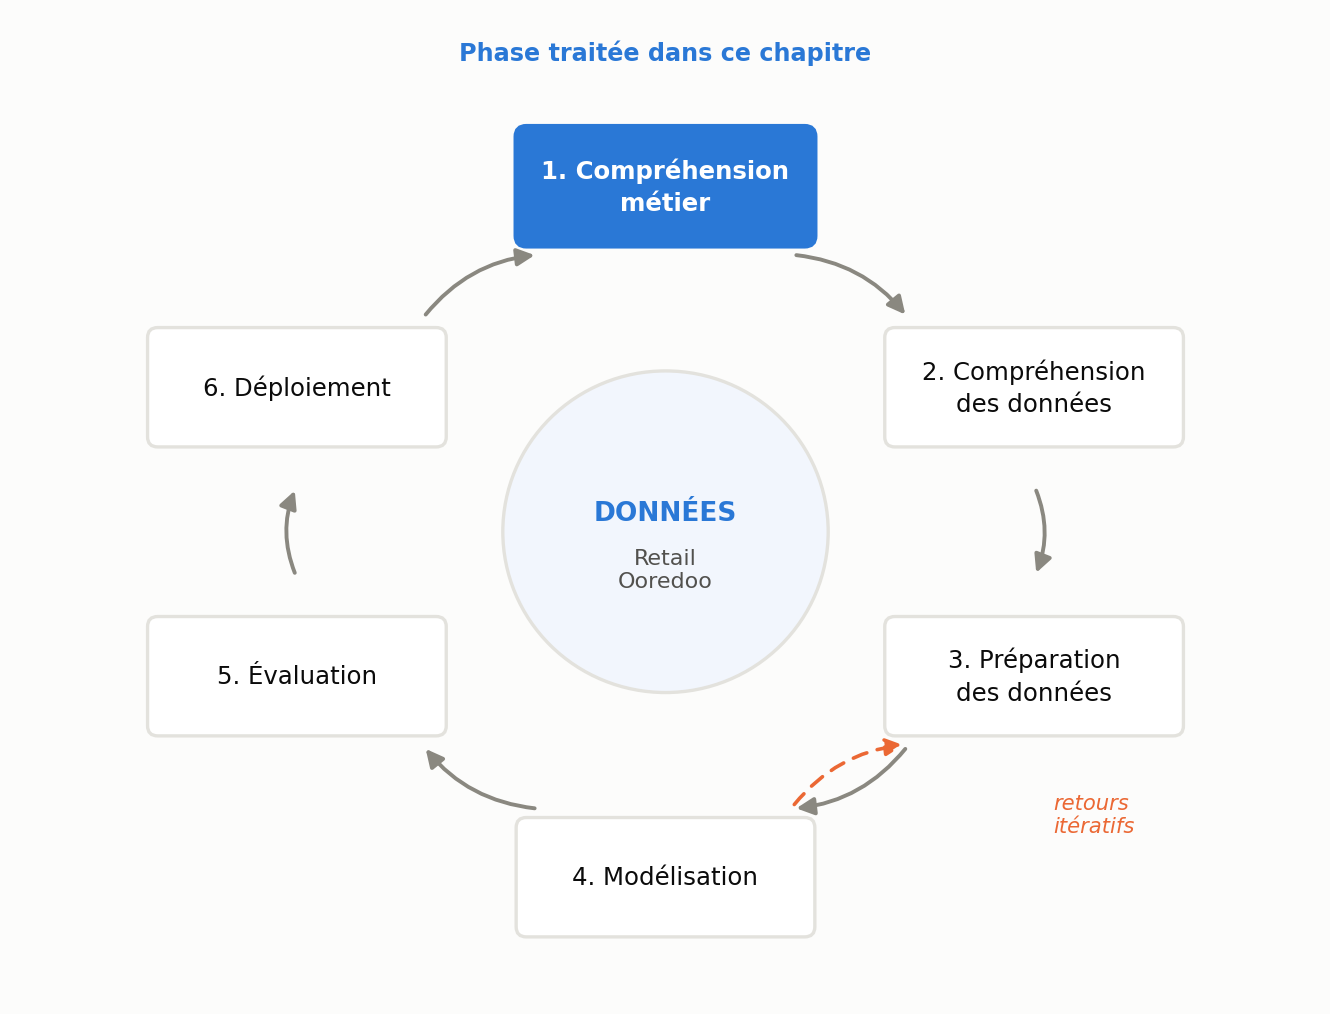
\includegraphics[width=0.68\textwidth]{img/fig_crispdm_phase1.png}
    \caption{Positionnement de la phase de compréhension métier dans le cycle CRISP-DM}
    \label{fig:crispdm-phase1-chap2}
\end{figure}

Le chapitre suit strictement les quatre tâches génériques définies par le guide de référence \cite{chapman2000crisp}, rappelées à la figure~\ref{fig:taches-phase1-chap2}. Nous \textbf{déterminons d'abord les objectifs métier} : ce que l'entreprise attend réellement du système et à quels critères elle jugera le résultat. Nous procédons ensuite à l'\textbf{évaluation de la situation} : inventaire des ressources, identification des acteurs, expression des exigences, hypothèses et contraintes, analyse des risques et de leurs parades, terminologie du domaine et analyse coûts-bénéfices. Nous \textbf{traduisons ensuite ces objectifs métier en objectifs de fouille de données}, assortis de critères de succès techniques mesurables — c'est le point d'articulation entre le métier et l'analyse. Nous modélisons enfin les besoins en UML \cite{booch2005uml}, puis nous \textbf{produisons le plan de projet}.

\begin{figure}[H]
    \centering
    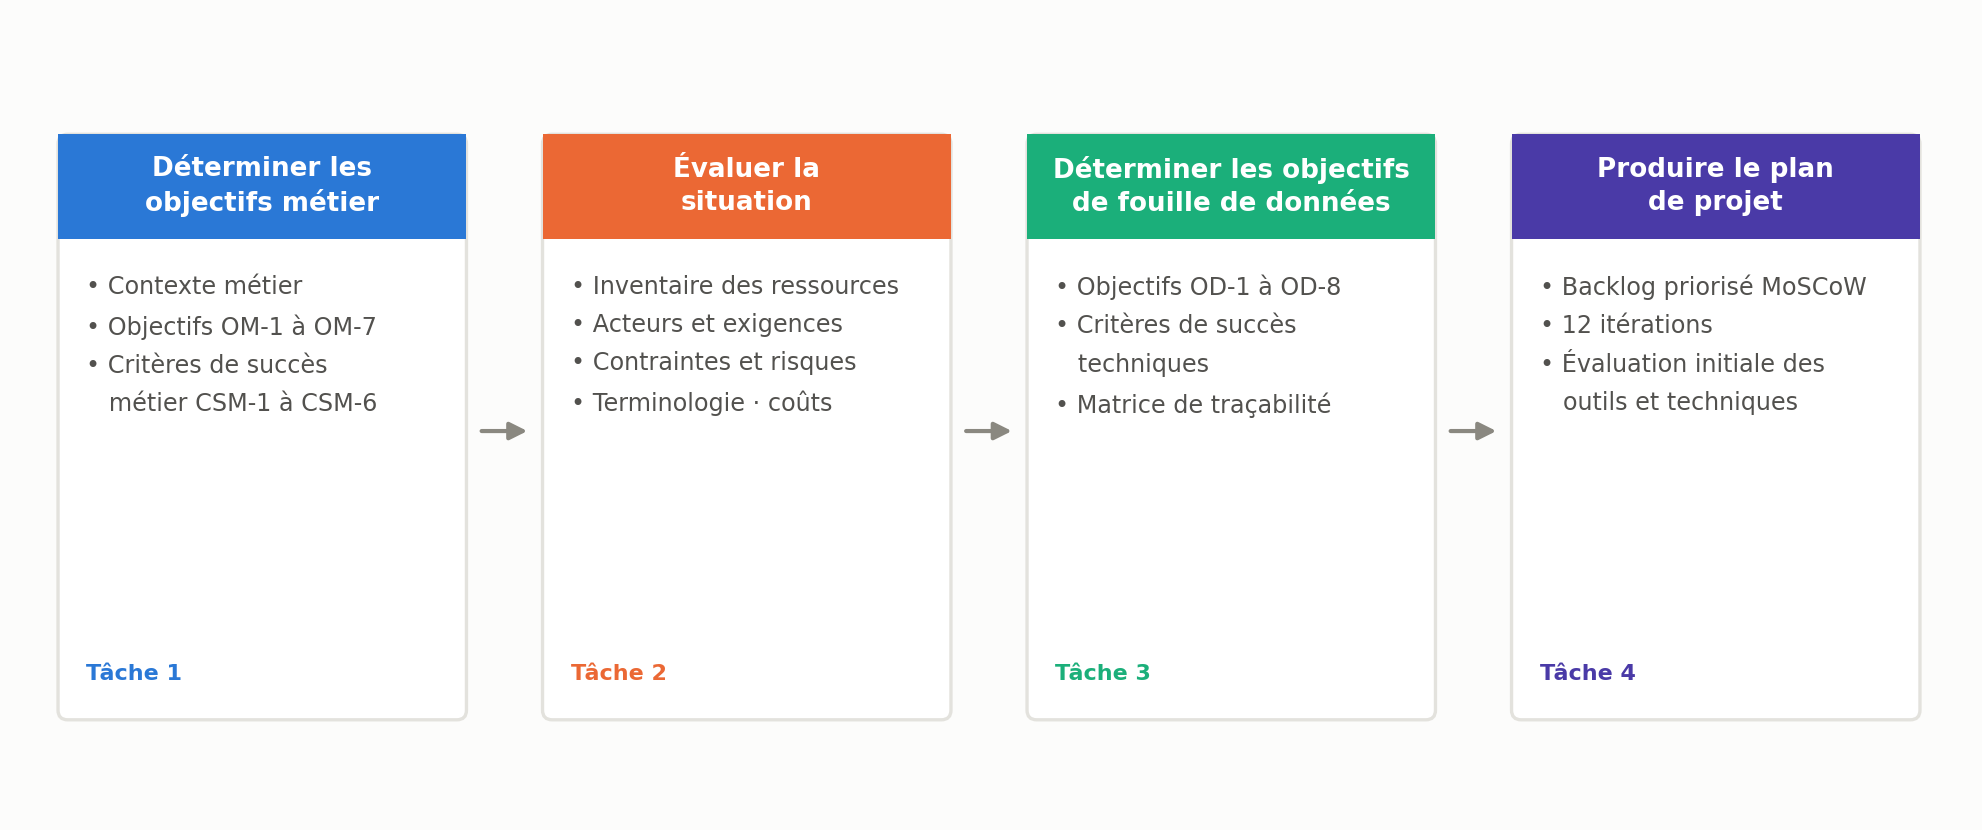
\includegraphics[width=\textwidth]{img/fig_taches_phase1.png}
    \caption{Les quatre tâches de la phase de compréhension métier et leurs livrables dans le projet}
    \label{fig:taches-phase1-chap2}
\end{figure}

La conception de la solution — architecture, agents, modèles — n'est délibérément pas abordée ici : elle relève de la phase de modélisation, traitée au chapitre~\ref{chap:modelisation}. Cette discipline est au cœur de CRISP-DM : on ne choisit pas une technique avant d'avoir formulé le problème qu'elle doit résoudre.

% ------------------------------------------------------------
\section{Détermination des objectifs métier}
% ------------------------------------------------------------

\subsection{Contexte métier}

Le point de vente Retail d'Ooredoo Tunisie fonctionne sur un cycle court : la journée. Un objectif de chiffre d'affaires est assigné à la boutique et réparti entre les conseillers ; il est atteint ou non le soir même. Entre les deux, la performance se joue heure par heure, sur un flux de clients dont le conseiller ne maîtrise ni le volume ni la composition, et sur un stock dont la disponibilité conditionne directement la vente : une référence absente du rayon est une vente perdue, pas différée. Cette asymétrie est bien documentée dans la littérature de prévision Retail \cite{fildes2022retail}, qui souligne que la rupture produit détruit une part de la demande au lieu de la reporter.

La figure~\ref{fig:processus-asis-chap2} représente le processus décisionnel actuel d'une journée en boutique et les quatre points de rupture qui en limitent l'efficacité. Elle met en évidence le défaut structurant : l'écart est constaté au moment où il n'est plus rattrapable.

\begin{figure}[H]
    \centering
    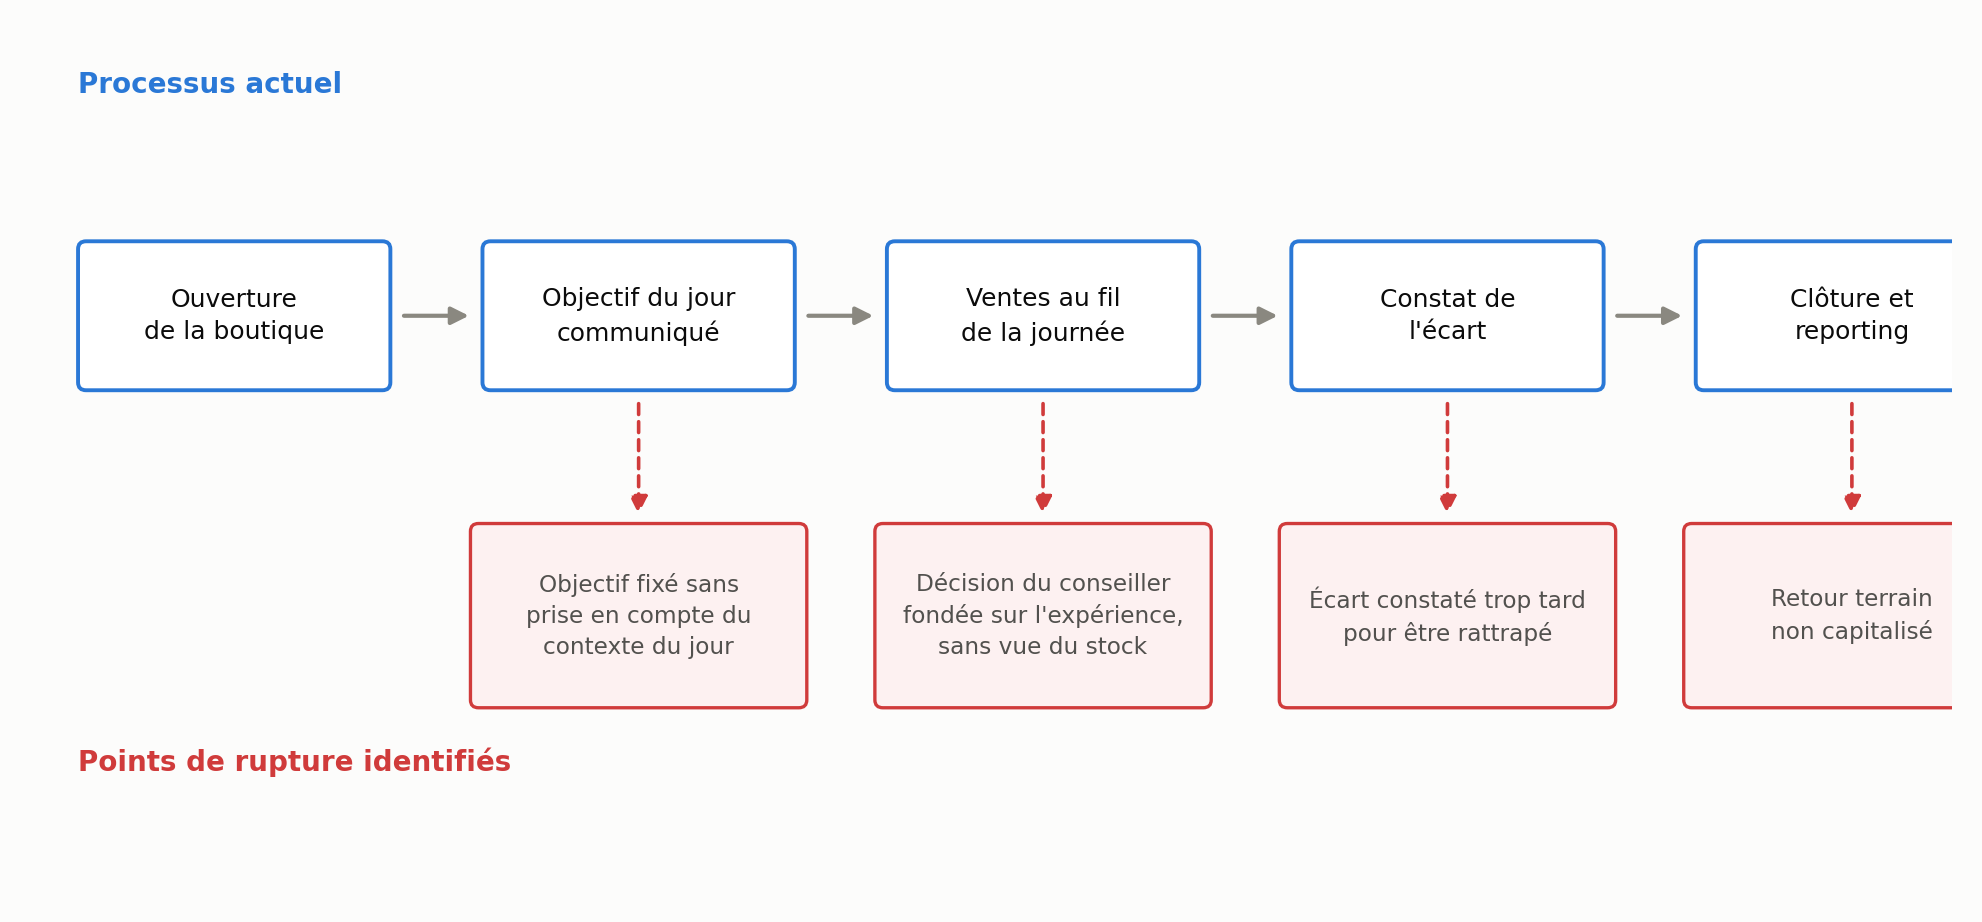
\includegraphics[width=\textwidth]{img/fig_processus_asis.png}
    \caption{Processus décisionnel actuel en point de vente et points de rupture identifiés}
    \label{fig:processus-asis-chap2}
\end{figure}

Deux leviers, aujourd'hui pilotés séparément, déterminent le résultat commercial :

\begin{itemize}[label=--]
    \item le \textbf{levier commercial} — quel produit proposer, avec quel argumentaire, à quel moment de la journée et à quel profil de client ;
    \item le \textbf{levier logistique} — quelle référence réapprovisionner, en quelle quantité et avec quelle urgence, compte tenu du délai fournisseur.
\end{itemize}

Ces deux leviers sont pourtant couplés, comme l'illustre la figure~\ref{fig:couplage-chap2} : une action commerciale poussant une référence en rupture imminente est contre-productive ; inversement, un réapprovisionnement décidé sans tenir compte de la dynamique commerciale immobilise de la trésorerie sur des produits qui ne tournent pas \cite{chopra2019supply}. Le projet part de ce constat : c'est le \textbf{croisement} des deux domaines qui porte la valeur, et non leur traitement isolé.

\begin{figure}[H]
    \centering
    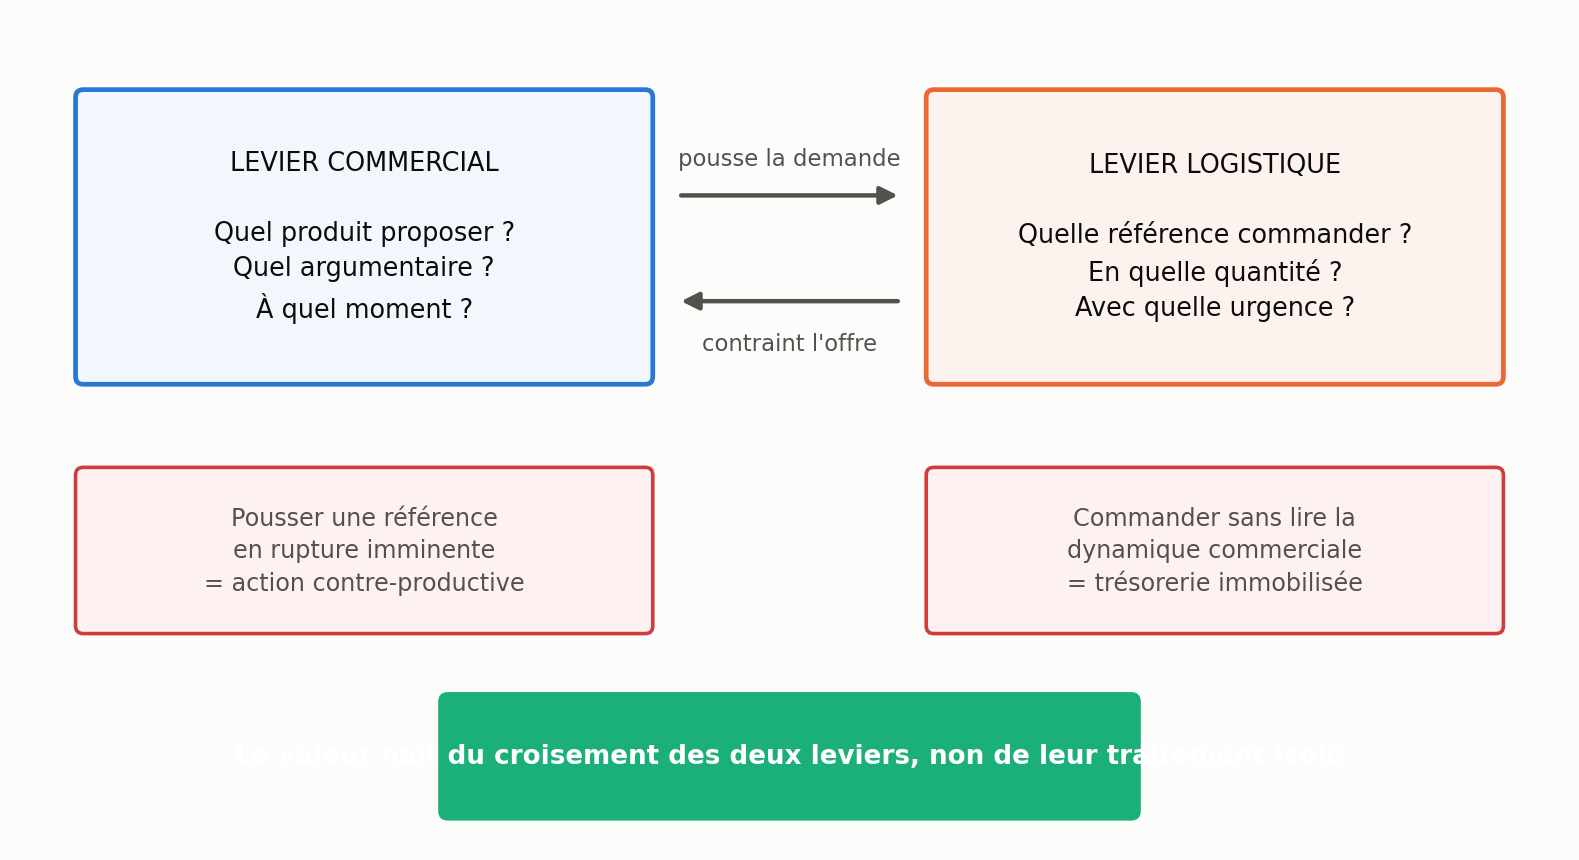
\includegraphics[width=0.92\textwidth]{img/fig_couplage_domaines.png}
    \caption{Couplage des leviers commercial et logistique}
    \label{fig:couplage-chap2}
\end{figure}

\subsection{Objectifs métier}

Les objectifs métier expriment ce que l'entreprise attend, en termes d'activité et non de technique. Ils ont été formulés à partir de l'analyse du contexte Retail présentée au chapitre~\ref{chap:cadre-general} et sont identifiés par un code \textbf{OM-\textit{n}} afin d'être traçables jusqu'aux critères d'évaluation du chapitre~\ref{chap:evaluation}.

Le tableau~\ref{tab:objectifs-metier-chap2} présente ces sept objectifs et l'enjeu que chacun porte pour l'entreprise.

\begin{longtable}{|P{1.4cm}|P{6.0cm}|P{6.6cm}|}
\hline
\rowcolor{red!75}
\textcolor{white}{\textbf{Code}} &
\textcolor{white}{\textbf{Objectif métier}} &
\textcolor{white}{\textbf{Enjeu pour l'entreprise}} \\
\hline
\endhead
\hline
\endfoot
\hline
\endlastfoot
OM-1 & Réduire l'écart entre le chiffre d'affaires réalisé et l'objectif journalier de la boutique & Améliorer le taux d'atteinte des objectifs commerciaux \\
\hline
OM-2 & Détecter la sous-performance pendant la journée de vente et non après sa clôture & Rendre l'écart rattrapable, donc actionnable \\
\hline
OM-3 & Réduire les ruptures de stock sur les références à forte rotation & Éviter la vente perdue et la dégradation de l'expérience client \\
\hline
OM-4 & Éviter le surstock et l'immobilisation de trésorerie sur les références à faible rotation & Optimiser le besoin en fonds de roulement du point de vente \\
\hline
OM-5 & Homogénéiser la qualité du conseil quel que soit le niveau d'expérience du conseiller & Réduire la dépendance à l'expertise individuelle et accélérer la montée en compétence \\
\hline
OM-6 & Accélérer et fiabiliser la décision de réapprovisionnement du manager & Réduire le délai entre la détection du besoin et l'engagement de la commande \\
\hline
OM-7 & Garantir que les conseils diffusés sont conformes aux règles commerciales et à l'état réel des stocks & Préserver la confiance des équipes et l'image de l'enseigne \\
\hline
\caption{Objectifs métier du projet}
\label{tab:objectifs-metier-chap2}
\end{longtable}

\subsection{Critères de succès métier}

Les critères de succès métier définissent à quelles conditions le projet sera jugé réussi \textit{par l'entreprise}. Ils sont volontairement exprimés du point de vue de l'usage, indépendamment de toute métrique technique : celles-ci sont introduites à la section~\ref{sec:objectifs-fouille}. Cette séparation, prescrite par le guide de référence \cite{chapman2000crisp}, évite la confusion fréquente entre un modèle performant et un projet utile.

\begin{longtable}{|P{1.8cm}|P{2.9cm}|P{9.3cm}|}
\hline
\rowcolor{red!75}
\textcolor{white}{\textbf{Code}} &
\textcolor{white}{\textbf{Dimension}} &
\textcolor{white}{\textbf{Critère de succès métier}} \\
\hline
\endhead
\hline
\endfoot
\hline
\endlastfoot
CSM-1 & Adoption & Le conseiller consulte et utilise les recommandations pendant son activité, sans allongement du temps de traitement d'un client \\
\hline
CSM-2 & Acceptation & Une majorité des propositions de réapprovisionnement soumises au manager est approuvée \\
\hline
CSM-3 & Anticipation & Les situations critiques sont signalées suffisamment tôt pour qu'une action corrective reste possible \\
\hline
CSM-4 & Confiance & Aucune recommandation diffusée ne contredit l'état réel du stock, les offres autorisées ou les règles commerciales \\
\hline
CSM-5 & Compréhension & L'utilisateur peut, pour toute recommandation, identifier les éléments chiffrés sur lesquels elle repose \\
\hline
CSM-6 & Autonomie de décision & Toute décision engageante reste soumise à l'arbitrage d'un responsable, qui conserve la capacité de rejeter la proposition \\
\hline
\caption{Critères de succès métier}
\label{tab:criteres-metier-chap2}
\end{longtable}

% ------------------------------------------------------------
\section{Évaluation de la situation}
% ------------------------------------------------------------

Cette deuxième tâche dresse un état des lieux factuel avant tout engagement technique : de quoi dispose-t-on, avec qui, sous quelles contraintes et face à quels risques.

\subsection{Inventaire des ressources}

\subsubsection{Ressources en données}

Le projet dispose d'un socle de données Retail couvrant les deux domaines. Le tableau~\ref{tab:ressources-donnees-chap2} en présente la nature et l'usage prévu ; leur exploration détaillée et leur contrôle de qualité relèvent de la phase de compréhension des données, traitée au chapitre~\ref{chap:donnees}.

\begin{longtable}{|P{3.0cm}|P{5.4cm}|P{6.0cm}|}
\hline
\rowcolor{red!75}
\textcolor{white}{\textbf{Domaine}} &
\textcolor{white}{\textbf{Données disponibles}} &
\textcolor{white}{\textbf{Usage prévu}} \\
\hline
\endhead
\hline
\endfoot
\hline
\endlastfoot
Ventes & Historique des transactions à granularité journalière et horaire, sur plusieurs années et plusieurs points de vente & Prévision du chiffre d'affaires, détection d'anomalies horaires, analyse de la performance \\
\hline
Référentiel commercial & Catalogue des produits et des boutiques, catégories, prix & Recommandation produit, valorisation des commandes \\
\hline
Objectifs & Objectifs commerciaux par boutique, par période et par conseiller & Calcul de l'écart et du taux d'atteinte \\
\hline
Stocks & Niveaux de stock par référence et par point de vente, historique des mouvements & Couverture, rotation, classification du risque \\
\hline
Approvisionnement & Délais fournisseurs, coûts de commande, historique des bons de commande & Point de commande, quantité économique de commande, priorisation \\
\hline
Contexte externe & Promotions et offres actives, événements locaux, jours fériés, conditions météorologiques & Enrichissement contextuel de l'analyse et de la recommandation \\
\hline
Connaissance métier & Scripts de vente, argumentaires, fiches produits et procédures & Base de connaissances interrogeable par l'assistant \\
\hline
Retour utilisateur & Décisions humaines : approbations, rejets et motifs & Boucle d'amélioration continue et mesure de l'acceptation \\
\hline
\caption{Inventaire des ressources en données}
\label{tab:ressources-donnees-chap2}
\end{longtable}

\subsubsection{Ressources matérielles}

Le développement a été réalisé sur un poste de travail unique, dont les caractéristiques figurent au tableau~\ref{tab:env-materiel-chap2}. Cette configuration s'est révélée suffisante pour exécuter simultanément le backend, le frontend, la base de données, le cache, la base vectorielle et les services annexes. Elle constitue toutefois une contrainte structurante, analysée à la section~\ref{sec:contraintes}.

\begin{longtable}{|P{4.5cm}|P{9.5cm}|}
\hline
\rowcolor{red!75}
\textcolor{white}{\textbf{Composant}} &
\textcolor{white}{\textbf{Caractéristiques}} \\
\hline
\endhead
\hline
\endfoot
\hline
\endlastfoot
Système d'exploitation & Microsoft Windows 10 Professionnel 22H2 (64 bits) \\
\hline
Processeur & Intel Core i7-10750H, 6 cœurs / 12 threads, 2,60 GHz \\
\hline
Mémoire vive & 16 Go \\
\hline
Stockage & SSD NVMe 256 Go (système et projet) + disque externe 500 Go (jeux de données et sauvegardes) \\
\hline
Carte graphique & NVIDIA GeForce GTX 1650 Ti, 4 Go de mémoire dédiée \\
\hline
\caption{Ressources matérielles disponibles}
\label{tab:env-materiel-chap2}
\end{longtable}

\subsubsection{Ressources humaines et expertise}

Le projet est mené individuellement dans le cadre d'un stage de fin d'études, avec l'accompagnement d'un encadrant académique et d'un encadrant professionnel. Cette configuration a une conséquence méthodologique directe : le projet cumule les rôles habituellement répartis dans une équipe data — ingénierie des données, modélisation, développement applicatif et intégration. Elle justifie le choix, opéré au chapitre~\ref{chap:cadre-general}, d'une méthodologie unique et légère plutôt que d'un cadre supposant une équipe structurée, tel que le \textit{Team Data Science Process} \cite{microsoft2020tdsp}.

\subsection{Identification des acteurs}

L'analyse du processus métier fait apparaître deux catégories d'acteurs : les acteurs humains, qui décident, et les agents logiciels, qui analysent et proposent. Un agent est ici entendu au sens classique des systèmes multi-agents \cite{wooldridge2009mas} : une entité autonome, dotée d'une perception de son environnement, d'objectifs propres et d'une capacité d'action ; sa déclinaison contemporaine fondée sur les modèles de langage est décrite par Guo et al. \cite{guo2024llmagents}.

La distinction entre les deux catégories est fondatrice pour le projet : la frontière qui les sépare définit précisément où s'arrête l'automatisation. La figure~\ref{fig:acteurs-chap2} en donne la cartographie.

\begin{figure}[H]
    \centering
    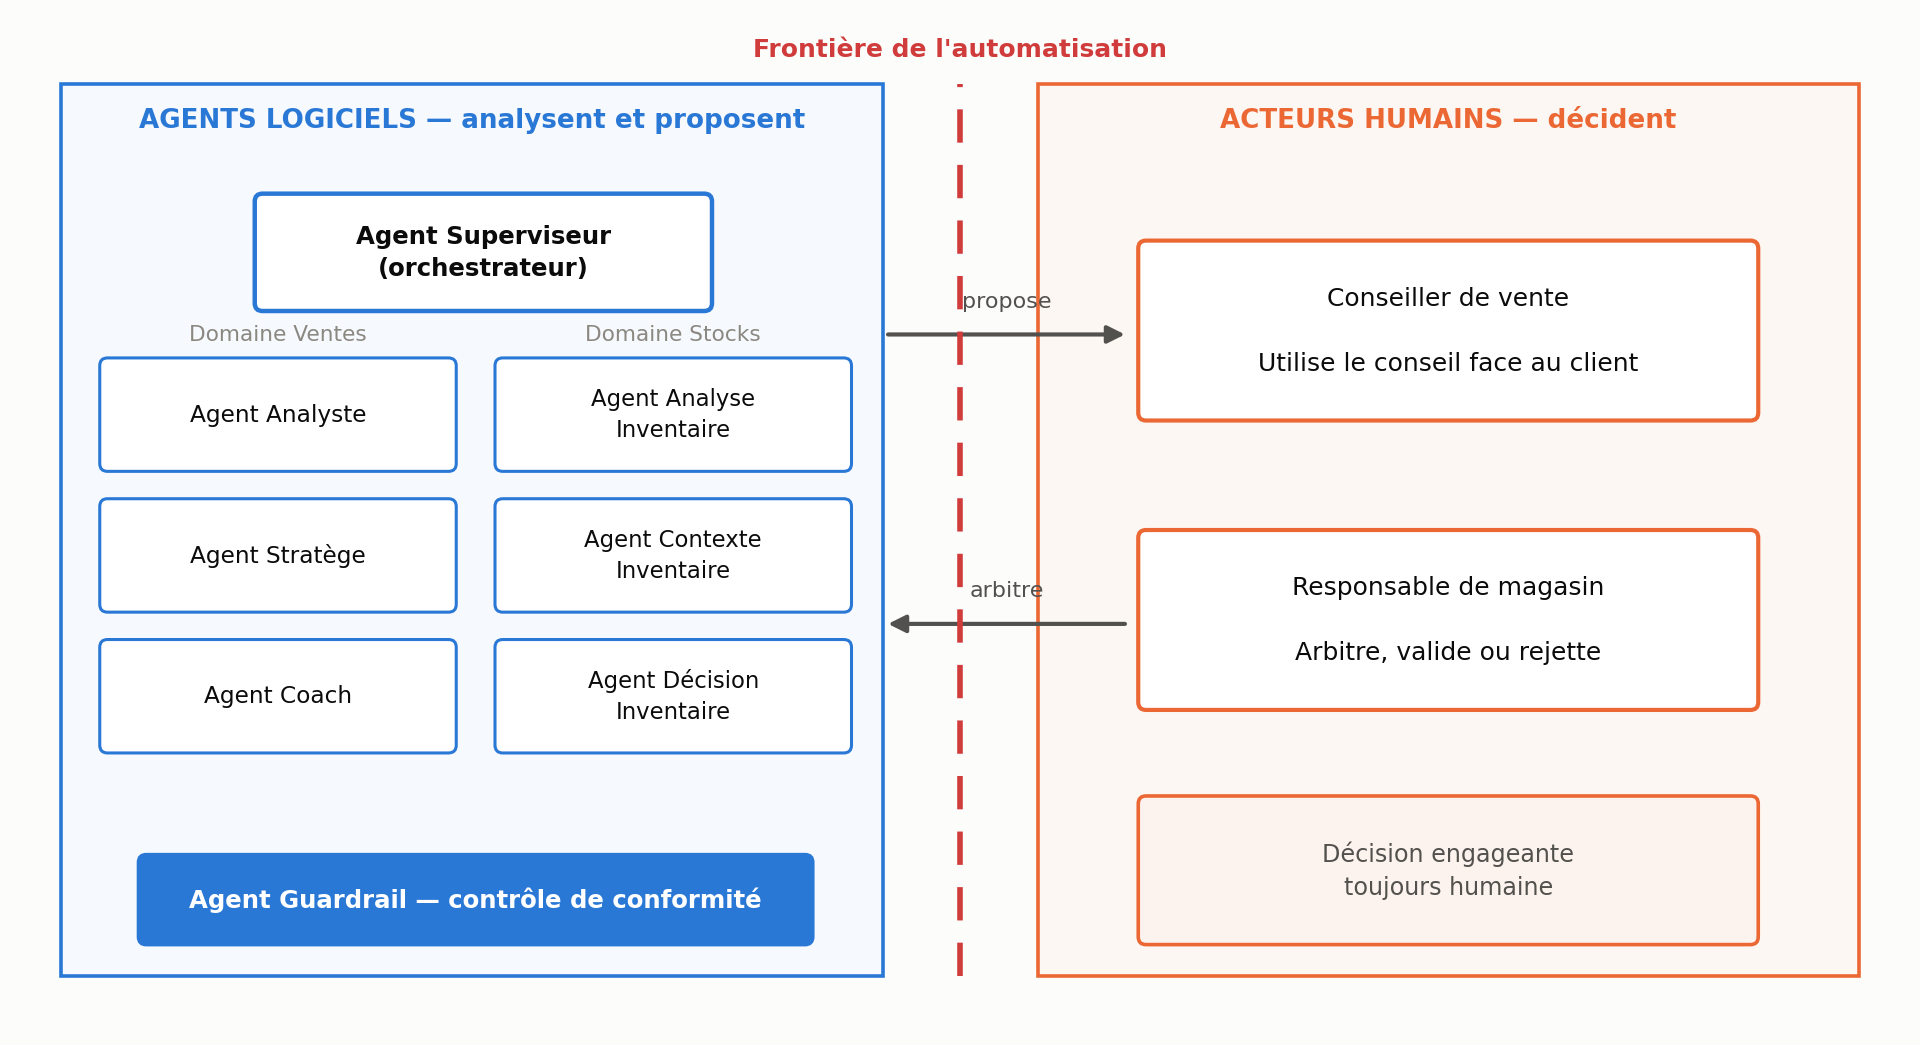
\includegraphics[width=\textwidth]{img/fig_cartographie_acteurs.png}
    \caption{Cartographie des acteurs et frontière de l'automatisation}
    \label{fig:acteurs-chap2}
\end{figure}

\subsubsection{Acteurs humains}

\begin{itemize}[label=--]
    \item \textbf{Le conseiller de vente} : utilisateur du volet coaching commercial. Il consulte sa performance du jour, reçoit alertes et recommandations produits, interroge l'assistant pendant la vente et signale les besoins de réapprovisionnement.
    \item \textbf{Le responsable de magasin (manager)} : utilisateur du volet supervision et gestion. Il suit la performance de la boutique et de son équipe, consulte l'état des stocks, arbitre les demandes des conseillers, approuve ou rejette les propositions de commande et supervise la qualité des recommandations produites.
\end{itemize}

L'accès aux fonctionnalités dépend du rôle : le conseiller est restreint aux données de sa propre boutique, le manager dispose d'une vue étendue et des fonctions de validation.

Le tableau~\ref{tab:acteurs-humains-chap2} décrit les acteurs humains du système et leurs prérogatives.

\begin{longtable}{|P{3.0cm}|P{4.6cm}|P{6.4cm}|}
\hline
\rowcolor{red!75}
\textcolor{white}{\textbf{Acteur}} &
\textcolor{white}{\textbf{Rôle}} &
\textcolor{white}{\textbf{Principales interactions attendues}} \\
\hline
\endhead
\hline
\endfoot
\hline
\endlastfoot
Conseiller de vente &
Utilisateur terrain du coaching commercial &
Consultation de sa performance et des alertes, dialogue avec l'assistant, demande de réapprovisionnement, suivi du statut de ses demandes \\
\hline
Responsable de magasin &
Superviseur de la boutique et décideur des approvisionnements &
Pilotage de la performance, consultation de l'état des stocks et du plan de commande, arbitrage des demandes, validation des propositions de commande, supervision de la qualité \\
\hline
\caption{Acteurs humains et responsabilités}
\label{tab:acteurs-humains-chap2}
\end{longtable}

\subsubsection{Acteurs logiciels : les agents intelligents}

Le système repose sur un ensemble d'agents spécialisés, chacun porteur d'une expertise et de ses propres outils de calcul. Leur rôle est présenté ici sous l'angle de la \textit{responsabilité métier} ; leur conception, leurs algorithmes et leur coordination relèvent du chapitre~\ref{chap:modelisation}.

Le tableau~\ref{tab:agents-intelligents-chap2} décrit les acteurs logiciels, c'est-à-dire les agents intelligents et leur rôle respectif.

\begin{longtable}{|P{4.2cm}|P{10.0cm}|}
\hline
\rowcolor{red!75}
\textcolor{white}{\textbf{Agent}} &
\textcolor{white}{\textbf{Responsabilité métier}} \\
\hline
\endhead
\hline
\endfoot
\hline
\endlastfoot
Agent Superviseur \newline (orchestrateur) &
Coordonner l'exécution des agents, assurer la circulation de l'information entre eux, arbitrer le déroulement du cycle et en conserver la trace. \\
\hline
Agent Analyste (Ventes) &
Établir le diagnostic commercial : chiffre d'affaires réalisé, écart à l'objectif, prévision de fin de journée et des prochaines heures, heures anormales, urgence du rattrapage. \\
\hline
Agent Stratège (Ventes) &
Élaborer les actions commerciales prioritaires à partir du diagnostic, du catalogue d'offres, de l'état des stocks et du contexte externe. \\
\hline
Agent Coach (Ventes) &
Formuler le message destiné au conseiller, hiérarchiser les produits à proposer avec leur justification, et répondre aux questions en langage naturel. \\
\hline
Agent Guardrail (contrôle) &
Vérifier la conformité de toute réponse avant diffusion et décider de son sort : diffusion, réécriture, escalade vers un humain ou blocage. \\
\hline
Agent Analyse Inventaire &
Établir le diagnostic de stock : couverture, rotation, niveau de risque par référence et paramètres de réapprovisionnement. \\
\hline
Agent Contexte Inventaire &
Enrichir ce diagnostic des facteurs susceptibles de modifier la demande : prévisions, promotions, événements, jours fériés, météo. \\
\hline
Agent Décision Inventaire &
Produire la décision de réapprovisionnement — commander, accélérer, maintenir, surveiller — avec quantité, confiance et justification, puis la soumettre à validation. \\
\hline
\caption{Agents intelligents et responsabilités métier}
\label{tab:agents-intelligents-chap2}
\end{longtable}

\subsection{Expression des exigences}

Les exigences traduisent les objectifs métier en fonctionnalités attendues et en qualités à garantir. Elles sont regroupées en huit familles fonctionnelles (\textbf{BF}) et sept familles non fonctionnelles (\textbf{BNF}), identifiées afin d'assurer la traçabilité jusqu'au backlog et jusqu'à l'évaluation.

\subsubsection{Exigences fonctionnelles}

\paragraph{BF-1 — Analyse et suivi des performances commerciales \textnormal{(OM-1, OM-2)}}

\begin{itemize}[label=--]
    \item BF-1.1 : suivre en temps réel le chiffre d'affaires du point de vente, l'objectif du jour, l'écart et le taux d'atteinte.
    \item BF-1.2 : restituer la performance heure par heure et identifier les heures en sous-performance.
    \item BF-1.3 : suivre la performance individuelle des conseillers (chiffre d'affaires, ventes, panier moyen, taux d'atteinte).
    \item BF-1.4 : détecter les anomalies de vente et qualifier leur degré d'urgence.
    \item BF-1.5 : présenter la répartition des ventes par catégorie et les références les plus performantes.
\end{itemize}

\paragraph{BF-2 — Prévision des ventes \textnormal{(OM-2)}}

\begin{itemize}[label=--]
    \item BF-2.1 : produire une prévision du chiffre d'affaires de fin de journée, assortie d'un intervalle de confiance.
    \item BF-2.2 : produire une prévision des prochaines heures afin d'anticiper l'évolution de l'activité.
    \item BF-2.3 : évaluer la faisabilité du rattrapage de l'objectif compte tenu du temps restant.
    \item BF-2.4 : rendre l'erreur du modèle vérifiable par un protocole de rétro-test \cite{hyndman2021fpp}.
\end{itemize}

\paragraph{BF-3 — Coaching commercial intelligent \textnormal{(OM-1, OM-5)}}

\begin{itemize}[label=--]
    \item BF-3.1 : recommander les produits à pousser, avec un score de priorité et une justification.
    \item BF-3.2 : fournir argumentaires et scripts de vente contextualisés, issus d'une base de connaissances métier.
    \item BF-3.3 : proposer un produit de substitution lorsque la référence demandée est indisponible et signaler les produits à éviter.
    \item BF-3.4 : adapter la recommandation à l'heure, à l'état de la boutique, aux offres actives et aux événements locaux.
    \item BF-3.5 : permettre au conseiller d'interroger l'assistant en langage naturel et recevoir la réponse progressivement.
    \item BF-3.6 : conserver l'historique des échanges afin de retrouver les recommandations antérieures.
\end{itemize}

\paragraph{BF-4 — Analyse et surveillance des stocks \textnormal{(OM-3, OM-4)}}

\begin{itemize}[label=--]
    \item BF-4.1 : suivre l'état des stocks par référence et par point de vente (quantité, couverture en jours, rotation).
    \item BF-4.2 : classer chaque référence selon son niveau de risque : rupture, couverture insuffisante, situation saine ou surstock.
    \item BF-4.3 : générer des alertes hiérarchisées sur les ruptures avérées et imminentes.
    \item BF-4.4 : restituer une vue de synthèse du portefeuille : santé du stock, références critiques, couverture moyenne.
\end{itemize}

\paragraph{BF-5 — Prévision de la demande \textnormal{(OM-3, OM-4)}}

\begin{itemize}[label=--]
    \item BF-5.1 : produire une prévision de la demande par référence à un horizon opérationnel.
    \item BF-5.2 : corriger cette prévision par les signaux de court terme : promotions, événements, saisonnalité.
    \item BF-5.3 : rendre la précision des prévisions de demande mesurable et publiable.
\end{itemize}

\paragraph{BF-6 — Décision de réapprovisionnement \textnormal{(OM-3, OM-4, OM-6)}}

\begin{itemize}[label=--]
    \item BF-6.1 : calculer stock de sécurité, point de commande et quantité économique de commande, en tenant compte du délai fournisseur et du niveau de service visé \cite{silver2016inventory,harris1913eoq}.
    \item BF-6.2 : produire une décision par référence — commander, accélérer, maintenir, surveiller — assortie d'un niveau de confiance.
    \item BF-6.3 : justifier la décision par les éléments chiffrés qui la fondent : couverture, demande prévue, délai, coût.
    \item BF-6.4 : consolider les décisions en un plan de commande chiffré à l'échelle du portefeuille.
\end{itemize}

\paragraph{BF-7 — Validation humaine et cycle de commande \textnormal{(OM-6, CSM-6)}}

\begin{itemize}[label=--]
    \item BF-7.1 : permettre au conseiller d'émettre une demande de réapprovisionnement depuis une alerte, et au manager de l'approuver ou de la rejeter avec un motif.
    \item BF-7.2 : matérialiser les propositions de l'agent sous forme de bons de commande suggérés, soumis à approbation avant tout engagement.
    \item BF-7.3 : suivre le cycle de vie d'un bon de commande, de la suggestion automatique jusqu'à la réception.
    \item BF-7.4 : soumettre à validation humaine les recommandations escaladées par le contrôle de conformité \cite{mosqueira2023human}.
    \item BF-7.5 : refléter en temps réel tout changement de statut dans l'interface.
\end{itemize}

\paragraph{BF-8 — Contrôle, supervision et amélioration continue \textnormal{(OM-7)}}

\begin{itemize}[label=--]
    \item BF-8.1 : vérifier chaque recommandation avant diffusion au regard des règles métier : disponibilité du produit, rupture imminente, origine de l'argumentaire, offres autorisées, éligibilité technique, niveau de confiance et montant engagé.
    \item BF-8.2 : substituer une réponse sûre lorsqu'une recommandation est bloquée, afin que l'utilisateur dispose toujours d'une réponse exploitable.
    \item BF-8.3 : orchestrer les agents des deux domaines et journaliser chaque cycle : agents invoqués, durées, erreurs.
    \item BF-8.4 : collecter le retour des utilisateurs — incitations suivies ou ignorées, décisions approuvées ou rejetées — et le réinjecter dans le raisonnement des agents.
    \item BF-8.5 : évaluer automatiquement la qualité des recommandations et publier les indicateurs correspondants \cite{zheng2023judge,es2024ragas}.
\end{itemize}

\subsubsection{Exigences non fonctionnelles}

Les exigences non fonctionnelles sont rattachées aux caractéristiques de qualité de la norme ISO/IEC 25010 \cite{iso25010}, afin d'en garantir la complétude et d'éviter le catalogue arbitraire.

Le tableau~\ref{tab:exigences-nf-chap2} recense les exigences non fonctionnelles, rattachées aux caractéristiques de qualité de la norme ISO/IEC 25010.

\begin{longtable}{|P{1.5cm}|P{3.0cm}|P{6.4cm}|P{3.0cm}|}
\hline
\rowcolor{red!75}
\textcolor{white}{\textbf{Code}} &
\textcolor{white}{\textbf{Exigence}} &
\textcolor{white}{\textbf{Contenu}} &
\textcolor{white}{\textbf{Caractéristique ISO 25010}} \\
\hline
\endhead
\hline
\endfoot
\hline
\endlastfoot
BNF-1 & Performance et réactivité & Produire analyses, prévisions, alertes et recommandations dans des délais compatibles avec un usage en boutique ; diffuser progressivement les réponses ; exécuter les traitements lourds hors du chemin critique & Efficacité de performance \\
\hline
BNF-2 & Fiabilité des recommandations & Garantir la cohérence avec l'état réel des stocks et les règles commerciales ; fonder les calculs décisionnels sur des méthodes déterministes plutôt que sur la génération de texte & Fiabilité · Exactitude fonctionnelle \\
\hline
BNF-3 & Disponibilité et robustesse & Maintenir les fonctions essentielles en cas d'indisponibilité d'un composant, par des mécanismes de repli explicites & Fiabilité (tolérance aux fautes) \\
\hline
BNF-4 & Sécurité et contrôle d'accès & Authentifier les utilisateurs, appliquer les droits par rôle et par boutique côté serveur, limiter la fréquence d'appel des points d'entrée sensibles & Sécurité \\
\hline
BNF-5 & Utilisabilité & Présenter l'information de manière claire et hiérarchisée, rester exploitable sur tablette, signaler les états de chargement et d'erreur & Utilisabilité \\
\hline
BNF-6 & Traçabilité et explicabilité & Conserver pour chaque recommandation sa justification, ses sources et le cycle qui l'a produite ; rendre les exécutions observables & Maintenabilité (analysabilité) \\
\hline
BNF-7 & Évaluabilité & Rendre la qualité des prévisions et des recommandations mesurable de façon reproductible & Maintenabilité (testabilité) \\
\hline
\caption{Exigences non fonctionnelles et rattachement à la norme ISO/IEC 25010}
\label{tab:exigences-nf-chap2}
\end{longtable}

\subsection{Hypothèses et contraintes}
\label{sec:contraintes}

\subsubsection{Hypothèses de travail}

\begin{itemize}[label=--]
    \item Les données de vente historiques sont représentatives du comportement commercial des points de vente étudiés.
    \item Les niveaux de stock enregistrés reflètent la disponibilité réelle en rayon, aux écarts d'inventaire près.
    \item Les objectifs commerciaux fournis constituent la référence de mesure de la performance.
    \item Les utilisateurs disposent d'un poste ou d'une tablette connectés pendant leur activité en boutique.
\end{itemize}

\subsubsection{Contraintes}

Le tableau~\ref{tab:contraintes-chap2} recense les hypothèses retenues et les contraintes qui s'imposent au projet.

\begin{longtable}{|P{3.0cm}|P{5.4cm}|P{6.0cm}|}
\hline
\rowcolor{red!75}
\textcolor{white}{\textbf{Nature}} &
\textcolor{white}{\textbf{Contrainte}} &
\textcolor{white}{\textbf{Conséquence sur le projet}} \\
\hline
\endhead
\hline
\endfoot
\hline
\endlastfoot
Temporelle & Six mois de stage, soit douze itérations de deux semaines & Périmètre borné par la méthode MoSCoW ; exclusion assumée de certaines fonctionnalités \\
\hline
Matérielle & Poste de développement unique, sans serveur d'inférence dédié & Les modèles lourds ne peuvent être exécutés localement en continu ; recours à des fournisseurs distants avec repli local \\
\hline
Économique & Absence de budget d'exploitation pour les modèles de langage & Recours prioritaire à des offres gratuites ou à faible coût, d'où la nécessité d'une cascade multi-fournisseurs \\
\hline
Organisationnelle & Absence d'accès à un ERP de production & Le cycle de commande est simulé jusqu'à la réception, sans interfaçage avec un système de facturation réel \\
\hline
Réglementaire & Protection des données commerciales et personnelles & Anonymisation des données sensibles, accès restreint par rôle et par boutique \\
\hline
Technique & Interface en français uniquement & L'internationalisation est exclue du périmètre, tout en conservant un modèle de vectorisation multilingue \cite{chen2024bge} pour préparer l'évolution \\
\hline
\caption{Contraintes du projet et conséquences}
\label{tab:contraintes-chap2}
\end{longtable}

\subsection{Risques et plans de contingence}

L'identification des risques est une tâche explicite de la phase de compréhension métier \cite{chapman2000crisp}. Chaque risque est ici associé à la parade prévue dès la conception, ce qui explique plusieurs choix d'architecture présentés au chapitre~\ref{chap:modelisation}. La figure~\ref{fig:risques-chap2} positionne les huit risques identifiés selon leur probabilité et leur impact ; le tableau~\ref{tab:risques-chap2} en détaille le traitement.

\begin{figure}[H]
    \centering
    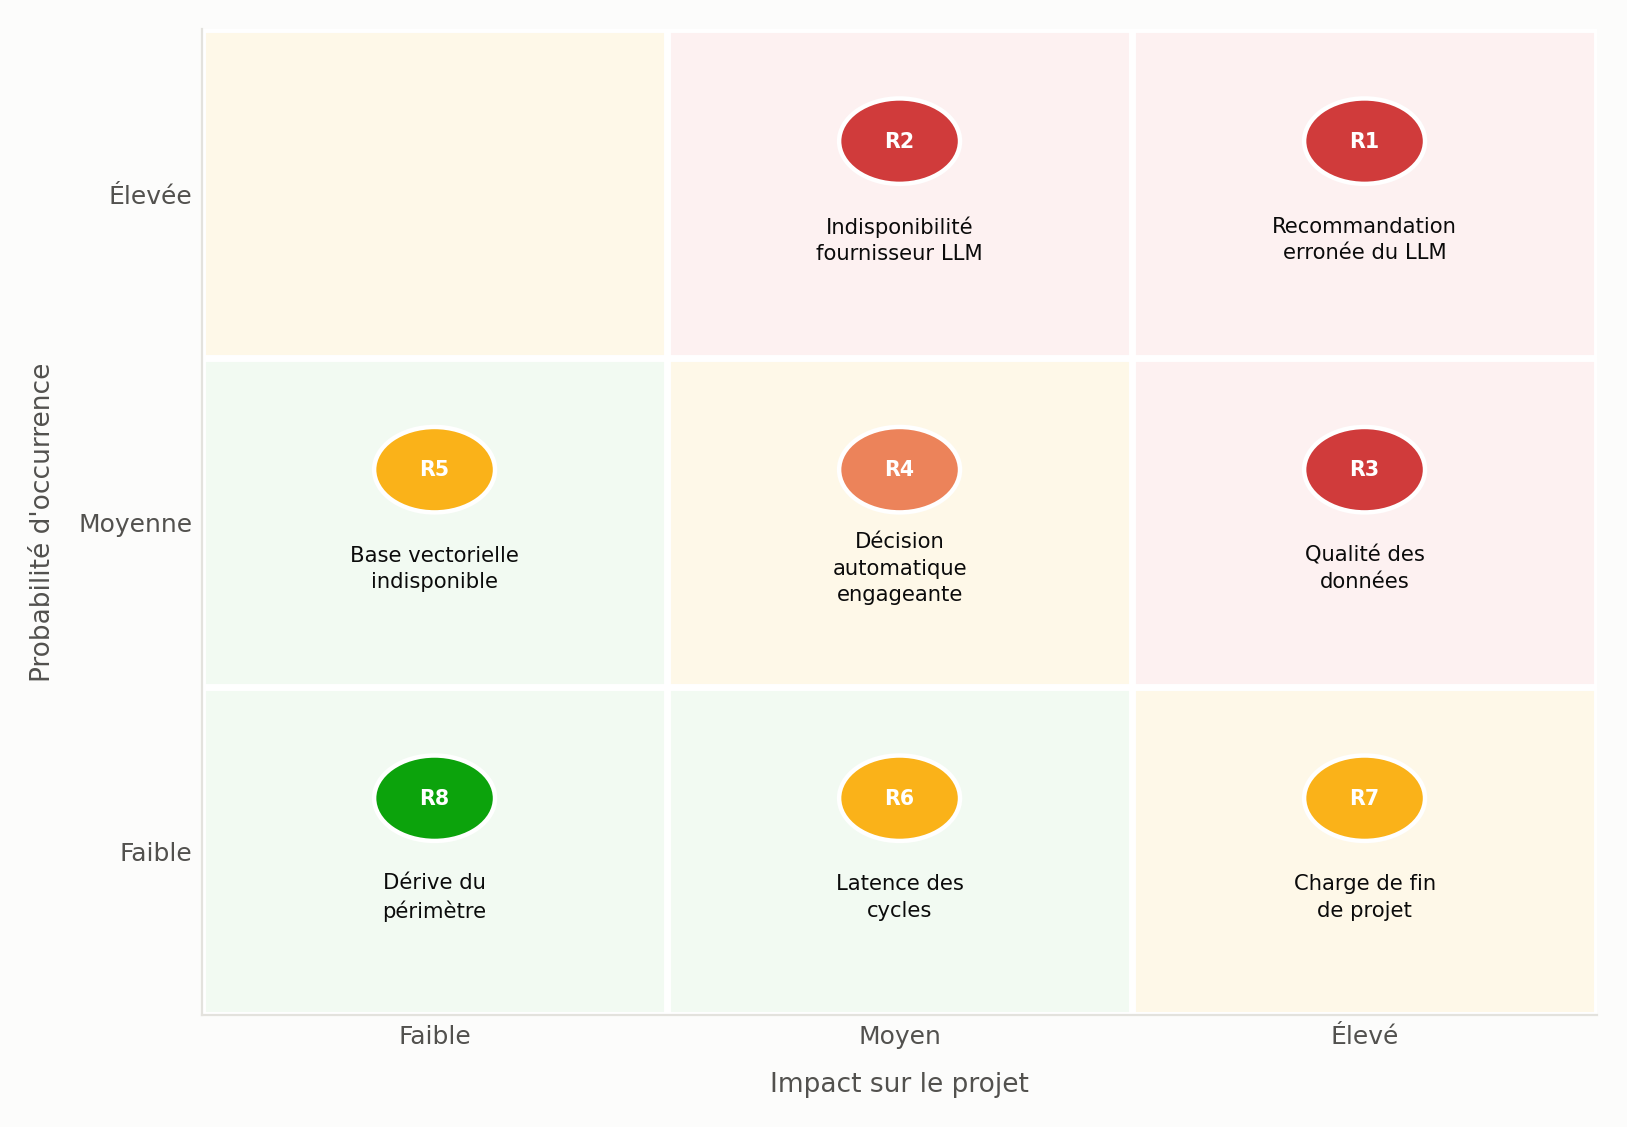
\includegraphics[width=0.82\textwidth]{img/fig_matrice_risques.png}
    \caption{Matrice des risques du projet (probabilité $\times$ impact)}
    \label{fig:risques-chap2}
\end{figure}

\begin{longtable}{|P{0.9cm}|P{3.4cm}|P{4.4cm}|P{4.8cm}|}
\hline
\rowcolor{red!75}
\textcolor{white}{\textbf{Réf.}} &
\textcolor{white}{\textbf{Risque}} &
\textcolor{white}{\textbf{Impact potentiel}} &
\textcolor{white}{\textbf{Plan de contingence}} \\
\hline
\endhead
\hline
\endfoot
\hline
\endlastfoot
R1 & Recommandation erronée produite par un modèle de langage \cite{ji2023hallucination} & Perte de confiance des utilisateurs, conseil commercial faux & Calculs décisionnels déterministes hors du modèle ; contrôle de conformité systématique avant diffusion ; citation obligatoire des sources \\
\hline
R2 & Indisponibilité ou quota épuisé d'un fournisseur de modèles & Interruption de l'assistant et des synthèses & Cascade multi-fournisseurs avec bascule automatique et repli sur une instance locale \\
\hline
R3 & Qualité insuffisante ou lacunes des données historiques & Prévisions non fiables, décisions faussées & Contrôle de qualité en phase de compréhension des données ; repli statistique lorsque l'historique est trop court \\
\hline
R4 & Décision automatique engageant l'entreprise & Commande injustifiée, immobilisation de trésorerie & Porte de validation humaine obligatoire avant tout engagement \cite{amershi2019guidelines} \\
\hline
R5 & Indisponibilité de la base vectorielle & Perte des argumentaires et des scripts & Repli sur un corpus local embarqué \\
\hline
R6 & Latence excessive d'un cycle multi-agents & Abandon de l'outil par le conseiller & Exécution parallèle des branches, mise en cache, évaluation de la qualité hors du chemin critique \\
\hline
R7 & Charge planifiée croissante en fin de projet & Fonctionnalités non livrées & Dépriorisation des items \textit{Should}, livraison incrémentale, réserve de capacité transverse \\
\hline
R8 & Dérive du périmètre & Dispersion et retard & Backlog priorisé MoSCoW et exclusions explicitement assumées \\
\hline
\caption{Analyse des risques et plans de contingence}
\label{tab:risques-chap2}
\end{longtable}

\subsection{Terminologie}

CRISP-DM recommande d'expliciter le vocabulaire du domaine afin d'éviter toute ambiguïté entre les acteurs métier et l'analyste \cite{chapman2000crisp}. Le tableau~\ref{tab:terminologie-chap2} définit les termes employés dans la suite du rapport.

\begin{longtable}{|P{3.6cm}|P{10.6cm}|}
\hline
\rowcolor{red!75}
\textcolor{white}{\textbf{Terme}} &
\textcolor{white}{\textbf{Définition retenue}} \\
\hline
\endhead
\hline
\endfoot
\hline
\endlastfoot
Référence (SKU) & Unité de gestion élémentaire du catalogue : un produit ou un service identifié de manière unique. \\
\hline
Taux d'atteinte & Rapport entre le chiffre d'affaires réalisé et l'objectif assigné, sur une même période. \\
\hline
Écart à l'objectif & Différence, en valeur ou en pourcentage, entre le réalisé et l'objectif ; il fonde le déclenchement des actions correctives. \\
\hline
Couverture de stock & Nombre de jours de vente que le stock disponible permet de couvrir au rythme de la demande observée. \\
\hline
Rotation & Vitesse à laquelle une référence s'écoule sur une période donnée. \\
\hline
Rupture & Situation dans laquelle le stock disponible d'une référence est nul ; la vente est perdue et non différée. \\
\hline
Délai de réapprovisionnement & Temps écoulé entre l'émission d'une commande et sa mise à disposition en rayon. \\
\hline
Stock de sécurité & Quantité tampon destinée à absorber la variabilité de la demande pendant le délai de réapprovisionnement \cite{axsater2015inventory}. \\
\hline
Point de commande & Niveau de stock déclenchant l'émission d'une nouvelle commande. \\
\hline
Quantité économique de commande & Quantité minimisant le coût total, par arbitrage entre coût de passation et coût de possession \cite{harris1913eoq}. \\
\hline
Niveau de service & Probabilité de ne pas subir de rupture pendant le délai de réapprovisionnement. \\
\hline
Agent & Composant logiciel autonome porteur d'une expertise, disposant de ses propres outils et contribuant à une décision collective \cite{wooldridge2009mas}. \\
\hline
Orchestration & Coordination de l'exécution des agents et de la circulation de l'information entre eux. \\
\hline
Garde-fou & Règle de contrôle appliquée à une réponse générée avant sa diffusion à l'utilisateur. \\
\hline
Validation humaine & Point d'arrêt du processus automatique où un responsable approuve, modifie ou rejette une proposition \cite{mosqueira2023human}. \\
\hline
Base de connaissances & Corpus documentaire métier indexé, interrogeable par similarité sémantique et par mots-clés \cite{lewis2020rag}. \\
\hline
Rétro-test & Protocole d'évaluation d'un modèle de prévision sur des périodes passées non utilisées pour son apprentissage \cite{hyndman2021fpp}. \\
\hline
\caption{Terminologie du domaine}
\label{tab:terminologie-chap2}
\end{longtable}

\subsection{Analyse coûts-bénéfices}

L'analyse coûts-bénéfices est conduite de manière qualitative, faute d'accès aux données financières consolidées de l'entreprise. Elle vise à vérifier que l'effort engagé est justifié par la valeur attendue.

Le tableau~\ref{tab:couts-benefices-chap2} met en regard les coûts engagés et les bénéfices attendus.

\begin{longtable}{|P{6.8cm}|P{7.4cm}|}
\hline
\rowcolor{red!75}
\textcolor{white}{\textbf{Coûts et efforts}} &
\textcolor{white}{\textbf{Bénéfices attendus}} \\
\hline
\endhead
\hline
\endfoot
\hline
\endlastfoot
Effort de développement sur six mois & Réduction de l'écart aux objectifs par une détection en cours de journée \\
\hline
Consommation d'appels aux modèles de langage & Réduction des ventes perdues par anticipation des ruptures \\
\hline
Effort d'intégration aux systèmes existants & Réduction de l'immobilisation de trésorerie liée au surstock \\
\hline
Accompagnement au changement des équipes terrain & Homogénéisation du conseil et montée en compétence accélérée \\
\hline
Maintenance des modèles et du corpus métier & Réduction du temps d'arbitrage du manager sur les réapprovisionnements \\
\hline
\caption{Analyse coûts-bénéfices qualitative}
\label{tab:couts-benefices-chap2}
\end{longtable}

% ------------------------------------------------------------
\section{Détermination des objectifs de fouille de données}
\label{sec:objectifs-fouille}
% ------------------------------------------------------------

Cette troisième tâche constitue le cœur méthodologique de la phase : elle traduit chaque objectif métier, exprimé en langage d'entreprise, en un ou plusieurs \textbf{objectifs de fouille de données} exprimés en termes d'analyse — nature du problème, sortie attendue, métrique d'évaluation \cite{chapman2000crisp}. Martínez-Plumed et al. \cite{martinez2021crisp} identifient précisément cette traduction comme le maillon le plus souvent escamoté des trajectoires de science des données réelles. La figure~\ref{fig:chaine-objectifs-chap2} en illustre le principe.

\begin{figure}[H]
    \centering
    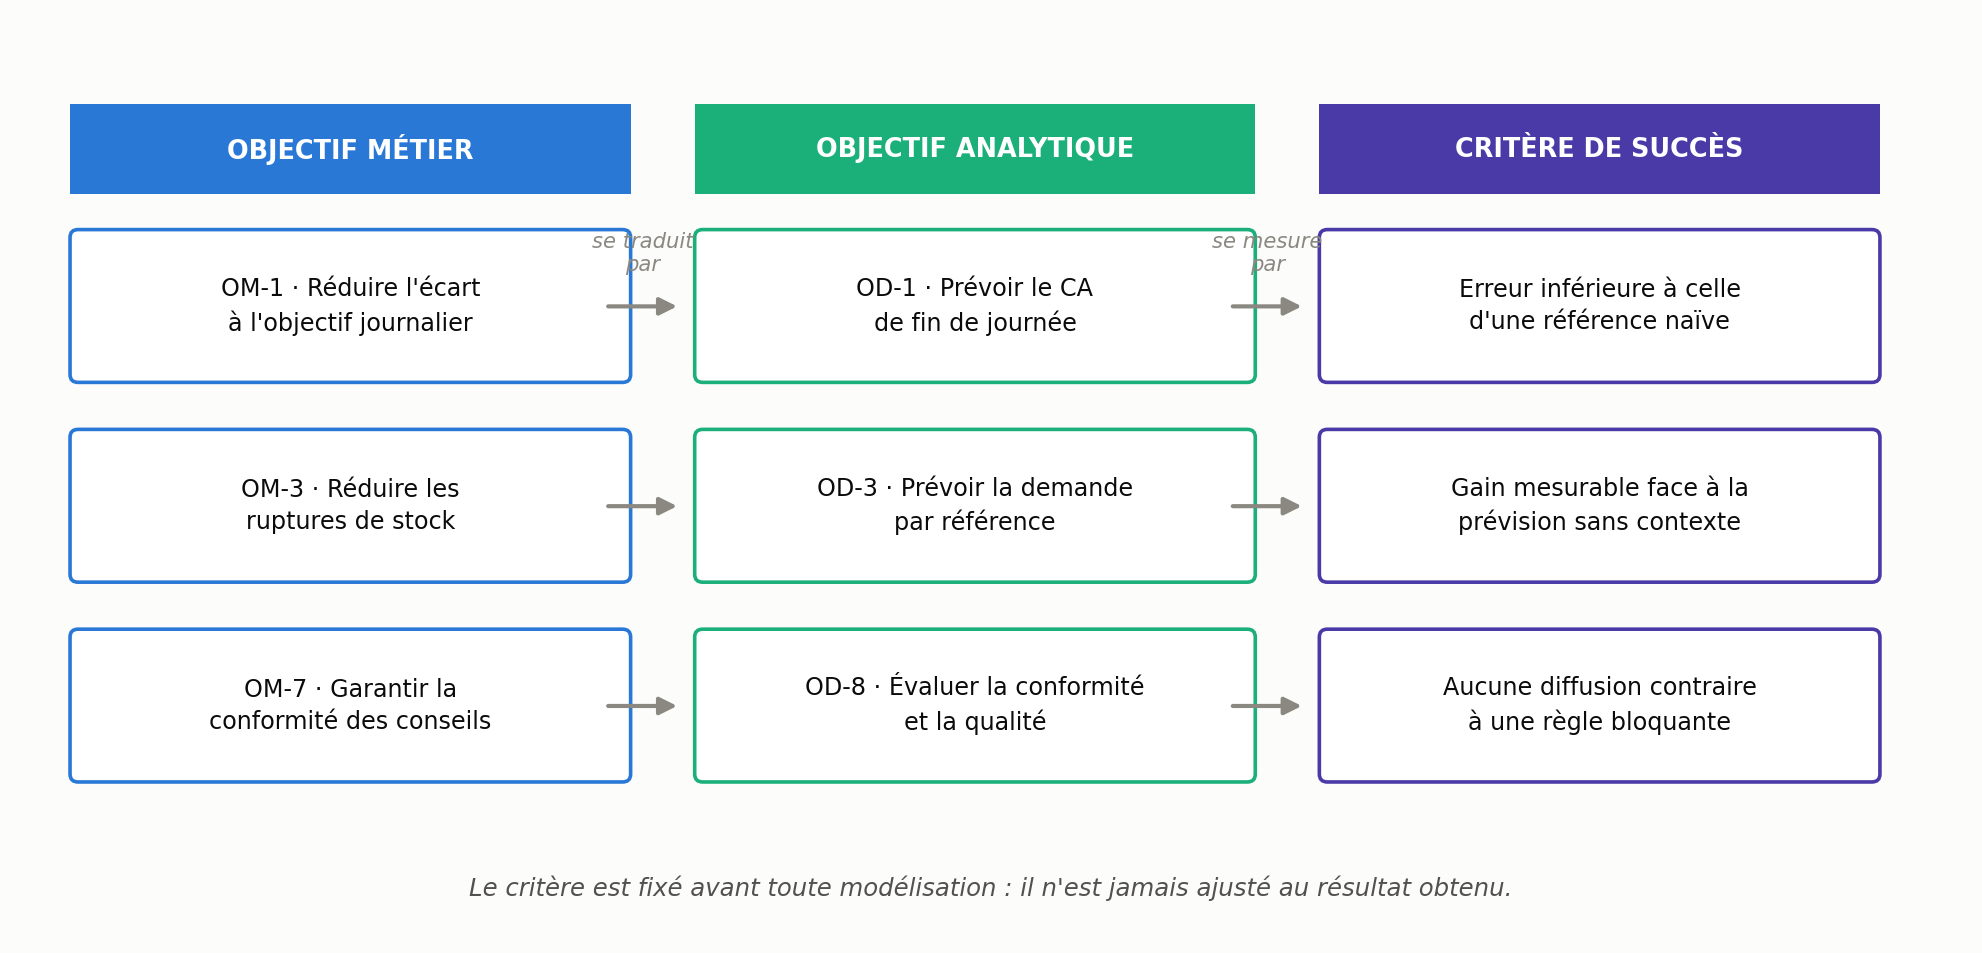
\includegraphics[width=\textwidth]{img/fig_chaine_objectifs.png}
    \caption{Chaîne de traduction : objectif métier, objectif analytique, critère de succès}
    \label{fig:chaine-objectifs-chap2}
\end{figure}

\subsection{Traduction des objectifs métier en objectifs analytiques}

\begingroup
\setlength{\tabcolsep}{3pt}
\renewcommand{\arraystretch}{1.15}
\small

Le tableau~\ref{tab:objectifs-fouille-chap2} présente cette traduction, objectif métier par objectif métier.

\begin{longtable}{|P{1.2cm}|P{4.0cm}|P{3.0cm}|P{5.6cm}|}
\hline
\rowcolor{red!75}
\textcolor{white}{\textbf{Réf.}} &
\textcolor{white}{\textbf{Objectif de fouille de données}} &
\textcolor{white}{\textbf{Nature du problème}} &
\textcolor{white}{\textbf{Sortie attendue}} \\
\hline
\endhead
\hline
\endfoot
\hline
\endlastfoot
OD-1 \newline \small (OM-1, OM-2) & Prévoir le chiffre d'affaires de fin de journée d'un point de vente & Régression sur série temporelle, saisonnalité hebdomadaire et profil intra-journalier & Valeur prévue et intervalle de confiance, actualisés en cours de journée \\
\hline
OD-2 \newline \small (OM-2) & Détecter les heures de sous-performance anormale & Détection d'anomalies par écart à un profil horaire attendu & Statut par heure et score d'écart normalisé \\
\hline
OD-3 \newline \small (OM-3, OM-4) & Prévoir la demande par référence à un horizon opérationnel & Régression sur série temporelle avec variables exogènes (promotions, événements, calendrier) & Demande prévue par référence et par jour \\
\hline
OD-4 \newline \small (OM-3, OM-4) & Classer chaque référence par niveau de risque de stock & Classification à partir de règles de gestion et de la demande prévue & Classe de risque : rupture, insuffisant, sain, surstock \\
\hline
OD-5 \newline \small (OM-6) & Déterminer la quantité et l'urgence de réapprovisionnement & Optimisation sous contrainte : coût, délai, niveau de service & Quantité recommandée, date de commande, priorité \\
\hline
OD-6 \newline \small (OM-1, OM-5) & Hiérarchiser les produits à proposer au client & Ordonnancement multicritère : marge, disponibilité, contexte, objectif & Liste ordonnée de produits, chacun assorti d'un score et d'une justification \\
\hline
OD-7 \newline \small (OM-5) & Retrouver l'argumentaire pertinent dans la connaissance métier & Recherche d'information hybride : sémantique et lexicale & Extraits documentaires classés, cités en référence \\
\hline
OD-8 \newline \small (OM-7) & Évaluer la conformité et la qualité d'une recommandation avant diffusion & Classification par règles, complétée d'une évaluation automatique a posteriori & Verdict de conformité et notes par critère de qualité \\
\hline
\caption{Traduction des objectifs métier en objectifs de fouille de données}
\label{tab:objectifs-fouille-chap2}
\end{longtable}
\endgroup

\subsection{Critères de succès techniques}

À chaque objectif analytique correspond un critère de succès technique, défini \textit{avant} toute modélisation afin d'éviter tout ajustement a posteriori du seuil au résultat obtenu. Ces critères constituent la référence d'évaluation utilisée au chapitre~\ref{chap:evaluation}. Le choix des métriques suit les recommandations de la littérature de prévision : mesure d'erreur relative agrégée et comparaison systématique à une méthode de référence naïve \cite{hyndman2021fpp,makridakis2020m4}.

\begin{longtable}{|P{1.3cm}|P{5.6cm}|P{7.1cm}|}
\hline
\rowcolor{red!75}
\textcolor{white}{\textbf{Réf.}} &
\textcolor{white}{\textbf{Métrique retenue}} &
\textcolor{white}{\textbf{Critère de succès}} \\
\hline
\endhead
\hline
\endfoot
\hline
\endlastfoot
OD-1 & Erreur absolue pondérée (WAPE) mesurée par rétro-test à origine glissante & Erreur inférieure à celle d'une référence naïve, et modèle retenu sur mesure comparative documentée \\
\hline
OD-2 & Cohérence des statuts horaires avec les écarts constatés & Toute heure dont l'écart dépasse le seuil défini est signalée, sans saturation d'alertes \\
\hline
OD-3 & Erreur absolue pondérée par référence & Amélioration mesurable par rapport à la prévision de référence sans correction contextuelle \\
\hline
OD-4 & Cohérence de la classification avec la couverture calculée & Aucune référence à stock nul classée autrement qu'en rupture \\
\hline
OD-5 & Taux d'acceptation des propositions par le manager & Majorité des propositions approuvées, motifs de rejet analysés \\
\hline
OD-6 & Pertinence des produits proposés au regard du contexte & Aucun produit indisponible dans la liste proposée \\
\hline
OD-7 & Fidélité aux sources et pertinence du contexte restitué & Chaque affirmation chiffrée rattachée à une source citée \\
\hline
OD-8 & Notes du juge automatique par critère et taux de blocage & Score de qualité conforme au seuil défini ; aucune diffusion contrevenant à une règle bloquante \\
\hline
\caption{Critères de succès techniques par objectif analytique}
\label{tab:criteres-succes-chap2}
\end{longtable}

Deux points méritent d'être soulignés. D'une part, les objectifs OD-1 à OD-5 relèvent de l'analyse quantitative classique et s'évaluent par des métriques d'erreur ; les objectifs OD-6 à OD-8 portent sur du texte et de l'ordonnancement, et exigent un protocole d'évaluation spécifique, combinant règles automatiques, juge automatique \cite{zheng2023judge} et retour humain. D'autre part, la réussite technique ne garantit pas la réussite métier : une prévision juste dont personne ne tient compte ne réduit aucun écart. C'est pourquoi les critères de succès métier du tableau~\ref{tab:criteres-metier-chap2} sont conservés distinctement et évalués séparément.

\subsection{Traçabilité des exigences}

La matrice suivante relie les exigences fonctionnelles aux objectifs métier et analytiques. Elle garantit qu'aucune exigence n'est orpheline et qu'aucun objectif n'est dépourvu de réalisation.

Le tableau~\ref{tab:tracabilite-chap2} établit cette traçabilité.

\begin{longtable}{|P{1.4cm}|P{4.6cm}|P{3.4cm}|P{4.2cm}|}
\hline
\rowcolor{red!75}
\textcolor{white}{\textbf{Exig.}} &
\textcolor{white}{\textbf{Intitulé}} &
\textcolor{white}{\textbf{Objectifs métier}} &
\textcolor{white}{\textbf{Objectifs analytiques}} \\
\hline
\endhead
\hline
\endfoot
\hline
\endlastfoot
BF-1 & Analyse et suivi des performances commerciales & OM-1, OM-2 & OD-2 \\
\hline
BF-2 & Prévision des ventes & OM-2 & OD-1 \\
\hline
BF-3 & Coaching commercial intelligent & OM-1, OM-5 & OD-6, OD-7 \\
\hline
BF-4 & Analyse et surveillance des stocks & OM-3, OM-4 & OD-4 \\
\hline
BF-5 & Prévision de la demande & OM-3, OM-4 & OD-3 \\
\hline
BF-6 & Décision de réapprovisionnement & OM-3, OM-4, OM-6 & OD-5 \\
\hline
BF-7 & Validation humaine et cycle de commande & OM-6 & OD-5, OD-8 \\
\hline
BF-8 & Contrôle, supervision et amélioration continue & OM-7 & OD-8 \\
\hline
\caption{Matrice de traçabilité exigences $\leftrightarrow$ objectifs}
\label{tab:tracabilite-chap2}
\end{longtable}

% ------------------------------------------------------------
\section{Modélisation des besoins}
% ------------------------------------------------------------

Afin de lever toute ambiguïté sur les exigences exprimées, celles-ci sont formalisées en UML \cite{booch2005uml}. Cette modélisation clôt l'expression du besoin : elle décrit \textit{ce que} le système doit permettre, sans préjuger de la manière dont il le réalisera.

\subsection{Diagramme de cas d'utilisation global}

Le conseiller et le manager héritent d'un acteur générique « Utilisateur authentifié » : les cas communs — authentification, consultation de la performance, dialogue avec l'assistant — lui sont associés, tandis que les cas de validation, de gestion des stocks et de supervision sont réservés au manager. Les agents interviennent comme acteur secondaire des cas qu'ils alimentent.

La figure~\ref{fig:cas-utilisation-global-chap2} présente le diagramme de cas d'utilisation global du système.

\begin{figure}[H]
    \centering
    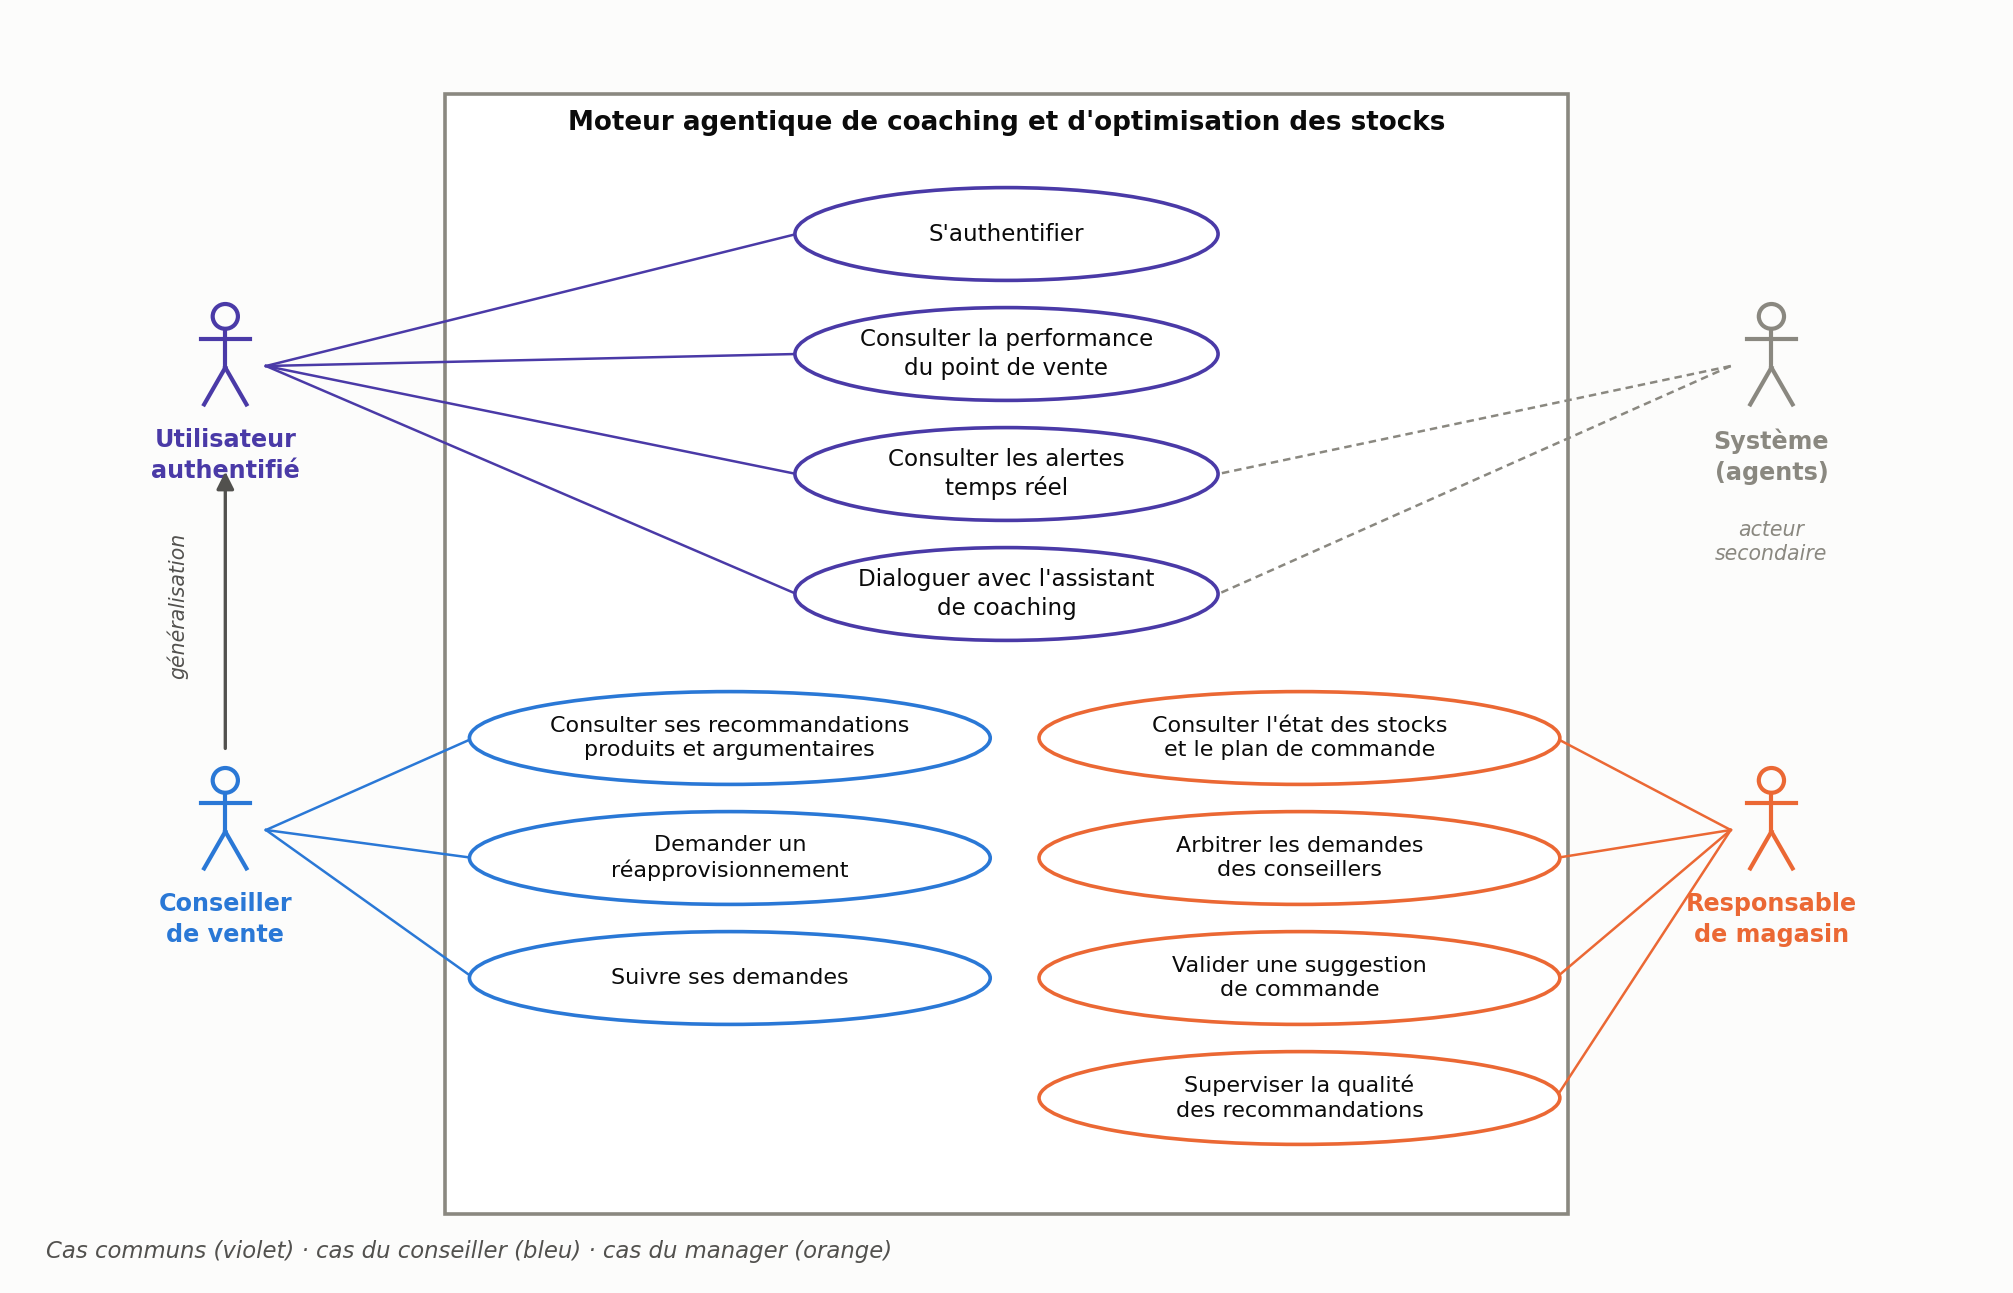
\includegraphics[width=\textwidth]{img/fig_cas_utilisation.png}
    \caption{Diagramme de cas d'utilisation global}
    \label{fig:cas-utilisation-global-chap2}
\end{figure}

Le tableau~\ref{tab:cas-utilisation-chap2} récapitule les cas d'utilisation principaux et les acteurs qui les déclenchent.

\begin{longtable}{|P{3.2cm}|P{5.4cm}|P{5.4cm}|}
\hline
\rowcolor{red!75}
\textcolor{white}{\textbf{Acteur}} &
\textcolor{white}{\textbf{Cas d'utilisation}} &
\textcolor{white}{\textbf{Exigences couvertes}} \\
\hline
\endhead
\hline
\endfoot
\hline
\endlastfoot
Utilisateur authentifié &
S'authentifier ; consulter la performance du point de vente ; consulter les alertes temps réel ; dialoguer avec l'assistant de coaching &
BF-1, BF-2, BF-3, BNF-4 \\
\hline
Conseiller de vente &
Consulter ses recommandations produits et argumentaires ; demander un réapprovisionnement ; suivre ses demandes &
BF-3, BF-7.1 \\
\hline
Responsable de magasin &
Consulter l'état des stocks et le plan de commande ; arbitrer les demandes des conseillers ; valider une suggestion de commande ; superviser la qualité des recommandations &
BF-4, BF-5, BF-6, BF-7, BF-8.5 \\
\hline
Système (agents) &
Analyser la performance ; analyser les stocks ; produire une recommandation ; contrôler la conformité ; suggérer un bon de commande &
BF-1 à BF-6, BF-8 \\
\hline
\caption{Cas d'utilisation par acteur}
\label{tab:cas-utilisation-chap2}
\end{longtable}

\subsection{Description des cas d'utilisation principaux}

Les cas d'utilisation les plus structurants sont décrits sous forme de fiches détaillées, selon le format proposé par Cockburn \cite{cockburn2001usecases} : acteurs, objectif, préconditions, scénario nominal, scénarios alternatifs, postconditions et exigences couvertes.

\subsubsection{Cas d'utilisation « Obtenir un conseil de vente »}

Le tableau~\ref{tab:cu-coach-chap2} en donne la fiche descriptive détaillée.

\begin{longtable}{|P{3.4cm}|P{10.8cm}|}
\hline
\rowcolor{red!75}
\textcolor{white}{\textbf{CU-01}} &
\textcolor{white}{\textbf{Obtenir un conseil de vente}} \\
\hline
\endhead
\hline
\endfoot
\hline
\endlastfoot
\textbf{Acteur principal} & Conseiller de vente \\
\hline
\textbf{Acteur secondaire} & Système (agents) \\
\hline
\textbf{Objectif} & Obtenir, pendant la vente, une recommandation argumentée adaptée à la situation de la boutique \\
\hline
\textbf{Préconditions} & L'utilisateur est authentifié et rattaché à une boutique ; les données de vente et de stock du jour sont disponibles \\
\hline
\textbf{Scénario nominal} &
1. Le conseiller pose une question en langage naturel ou sélectionne une suggestion contextuelle. \newline
2. Le système établit le diagnostic commercial, consulte la connaissance métier, collecte le contexte et vérifie l'état des stocks. \newline
3. Ces éléments sont consolidés en une analyse unique. \newline
4. Le système formule la réponse, hiérarchise les produits à proposer et cite ses sources. \newline
5. La conformité de la réponse est contrôlée. \newline
6. La réponse est diffusée progressivement au conseiller, avec son statut de vérification. \\
\hline
\textbf{Scénarios alternatifs} &
5a. Règle mineure enfreinte : la réponse est reformulée avant diffusion. \newline
5b. Confiance insuffisante ou montant engagé élevé : la réponse est escaladée vers une validation humaine. \newline
5c. Produit indisponible ou offre non autorisée : la réponse est bloquée et remplacée par une réponse sûre. \\
\hline
\textbf{Postconditions} & Le conseiller dispose d'une recommandation vérifiée ; le cycle, ses sources et le verdict sont journalisés \\
\hline
\textbf{Exigences} & BF-3, BF-8.1, BF-8.2, BNF-1, BNF-6 \\
\hline
\caption{Fiche descriptive du cas d'utilisation « Obtenir un conseil de vente »}
\label{tab:cu-coach-chap2}
\end{longtable}

\subsubsection{Cas d'utilisation « Demander un réapprovisionnement »}

Le tableau~\ref{tab:cu-demande-chap2} en donne la fiche descriptive détaillée.

\begin{longtable}{|P{3.4cm}|P{10.8cm}|}
\hline
\rowcolor{red!75}
\textcolor{white}{\textbf{CU-02}} &
\textcolor{white}{\textbf{Demander un réapprovisionnement}} \\
\hline
\endhead
\hline
\endfoot
\hline
\endlastfoot
\textbf{Acteurs} & Conseiller de vente (demandeur), responsable de magasin (décideur) \\
\hline
\textbf{Objectif} & Faire remonter au manager le besoin de réapprovisionnement d'une référence en rupture ou en risque \\
\hline
\textbf{Préconditions} & Une alerte de rupture ou de risque est active sur une référence de la boutique \\
\hline
\textbf{Scénario nominal} &
1. Le conseiller sélectionne l'alerte et demande le réapprovisionnement en indiquant la quantité souhaitée. \newline
2. Le système enregistre la demande avec son motif, son auteur et son horodatage, au statut « en attente ». \newline
3. Le manager consulte la liste des demandes et arbitre. \newline
4. Il approuve ou rejette la demande, éventuellement avec une note destinée au conseiller. \newline
5. Le statut est mis à jour et devient immédiatement visible dans l'espace du conseiller. \\
\hline
\textbf{Scénario alternatif} &
4a. En cas de rejet, le motif est conservé et alimente le retour d'expérience exploité par les agents. \\
\hline
\textbf{Postconditions} & La demande est tracée avec sa décision ; le conseiller connaît le sort de sa demande \\
\hline
\textbf{Exigences} & BF-7.1, BF-7.5, BF-8.4, BNF-4 \\
\hline
\caption{Fiche descriptive du cas d'utilisation « Demander un réapprovisionnement »}
\label{tab:cu-demande-chap2}
\end{longtable}

\subsubsection{Cas d'utilisation « Valider une suggestion de commande »}

Le tableau~\ref{tab:cu-po-chap2} en donne la fiche descriptive détaillée.

\begin{longtable}{|P{3.4cm}|P{10.8cm}|}
\hline
\rowcolor{red!75}
\textcolor{white}{\textbf{CU-03}} &
\textcolor{white}{\textbf{Valider une suggestion de commande}} \\
\hline
\endhead
\hline
\endfoot
\hline
\endlastfoot
\textbf{Acteur principal} & Responsable de magasin \\
\hline
\textbf{Acteur secondaire} & Système (agents) \\
\hline
\textbf{Objectif} & Décider du sort d'un bon de commande proposé automatiquement par le système \\
\hline
\textbf{Préconditions} & Une recommandation de réapprovisionnement a donné lieu à un bon de commande au statut « suggestion automatique » \\
\hline
\textbf{Scénario nominal} &
1. Le manager consulte les bons de commande, en vue liste ou en vue Kanban. \newline
2. Il ouvre la fiche : quantité, prix unitaire, délai de livraison prévu, priorité, niveau de confiance et justification. \newline
3. Il approuve la suggestion, qui entre alors dans le circuit de commande. \newline
4. Il fait progresser le bon de commande le long de son cycle jusqu'à la réception. \newline
5. Chaque transition est diffusée en temps réel aux utilisateurs connectés. \\
\hline
\textbf{Scénarios alternatifs} &
3a. Le manager rejette la suggestion : le bon est annulé et le motif conservé. \newline
4a. La réception est partielle : le bon reste ouvert jusqu'à complétion. \\
\hline
\textbf{Postconditions} & Le cycle de la commande est tracé de bout en bout ; l'issue alimente la mesure du taux d'acceptation \\
\hline
\textbf{Exigences} & BF-6, BF-7.2, BF-7.3, BF-7.5, BF-8.4 \\
\hline
\caption{Fiche descriptive du cas d'utilisation « Valider une suggestion de commande »}
\label{tab:cu-po-chap2}
\end{longtable}

\subsection{Diagrammes de séquence}

Deux scénarios représentatifs sont détaillés : l'un déclenché par l'utilisateur, l'autre par le système. Ils sont présentés au niveau des interactions métier ; leur réalisation technique est décrite au chapitre~\ref{chap:modelisation}.

Le premier scénario (figure~\ref{fig:sequence-coach-chap2}) décrit le dialogue avec l'assistant de coaching. Il fait apparaître trois propriétés attendues du système : la consultation conjointe des analyses de vente, de la connaissance métier et de l'état des stocks ; le contrôle systématique de la réponse avant sa diffusion ; et la restitution progressive, qui réduit le temps d'attente perçu.

\begin{figure}[H]
    \centering
    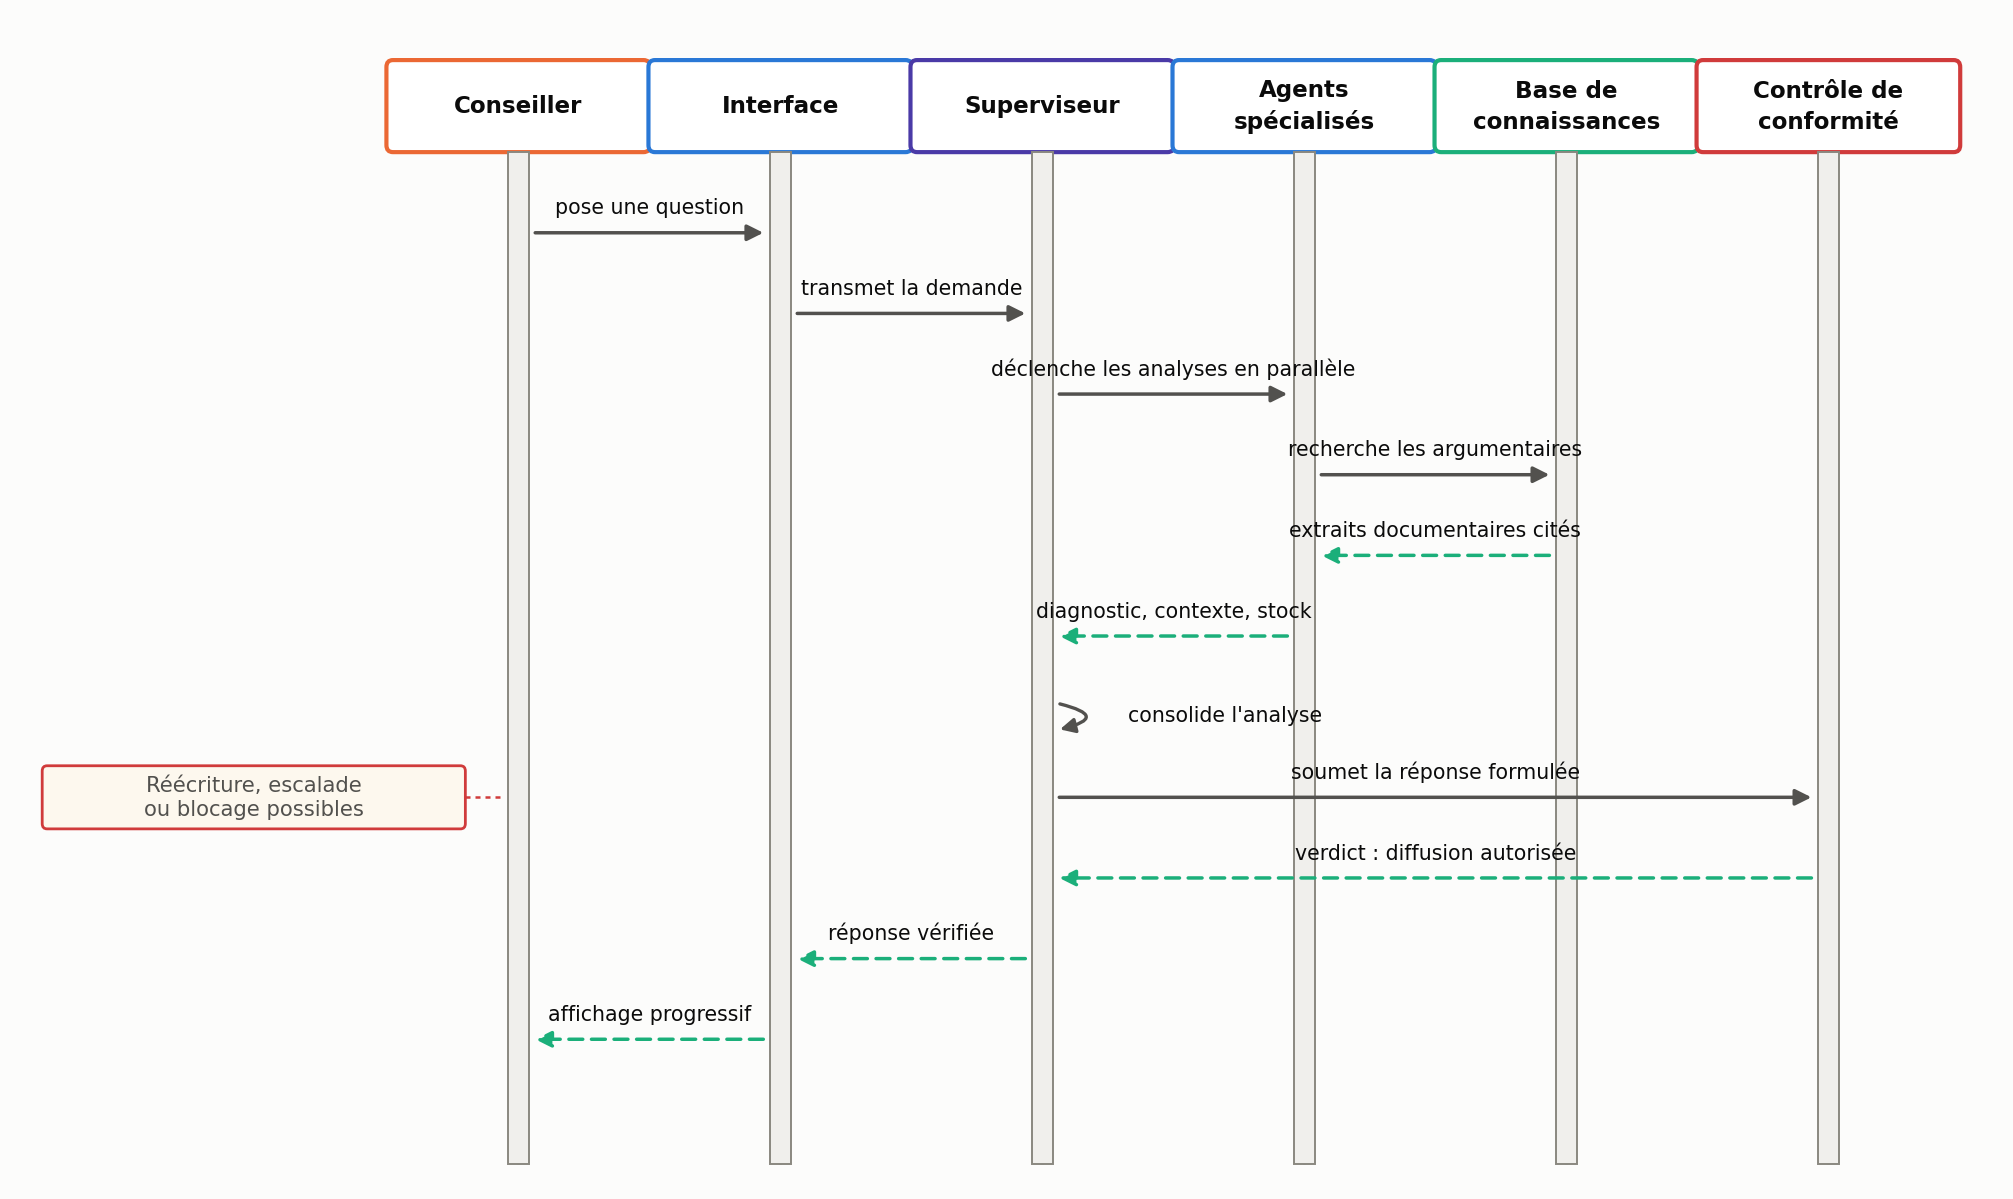
\includegraphics[width=\textwidth]{img/fig_sequence_coach.png}
    \caption{Diagramme de séquence — dialogue avec l'assistant de coaching}
    \label{fig:sequence-coach-chap2}
\end{figure}

Le second scénario (figure~\ref{fig:sequence-reappro-chap2}) illustre un cycle proactif : la détection d'une situation critique de stock déclenche, sans sollicitation humaine, l'analyse, l'enrichissement contextuel et la décision, jusqu'à la création d'une suggestion de commande. La chaîne s'interrompt volontairement devant la porte de validation : l'engagement d'une commande demeure une décision du manager, conformément à l'exigence CSM-6.

\begin{figure}[H]
    \centering
    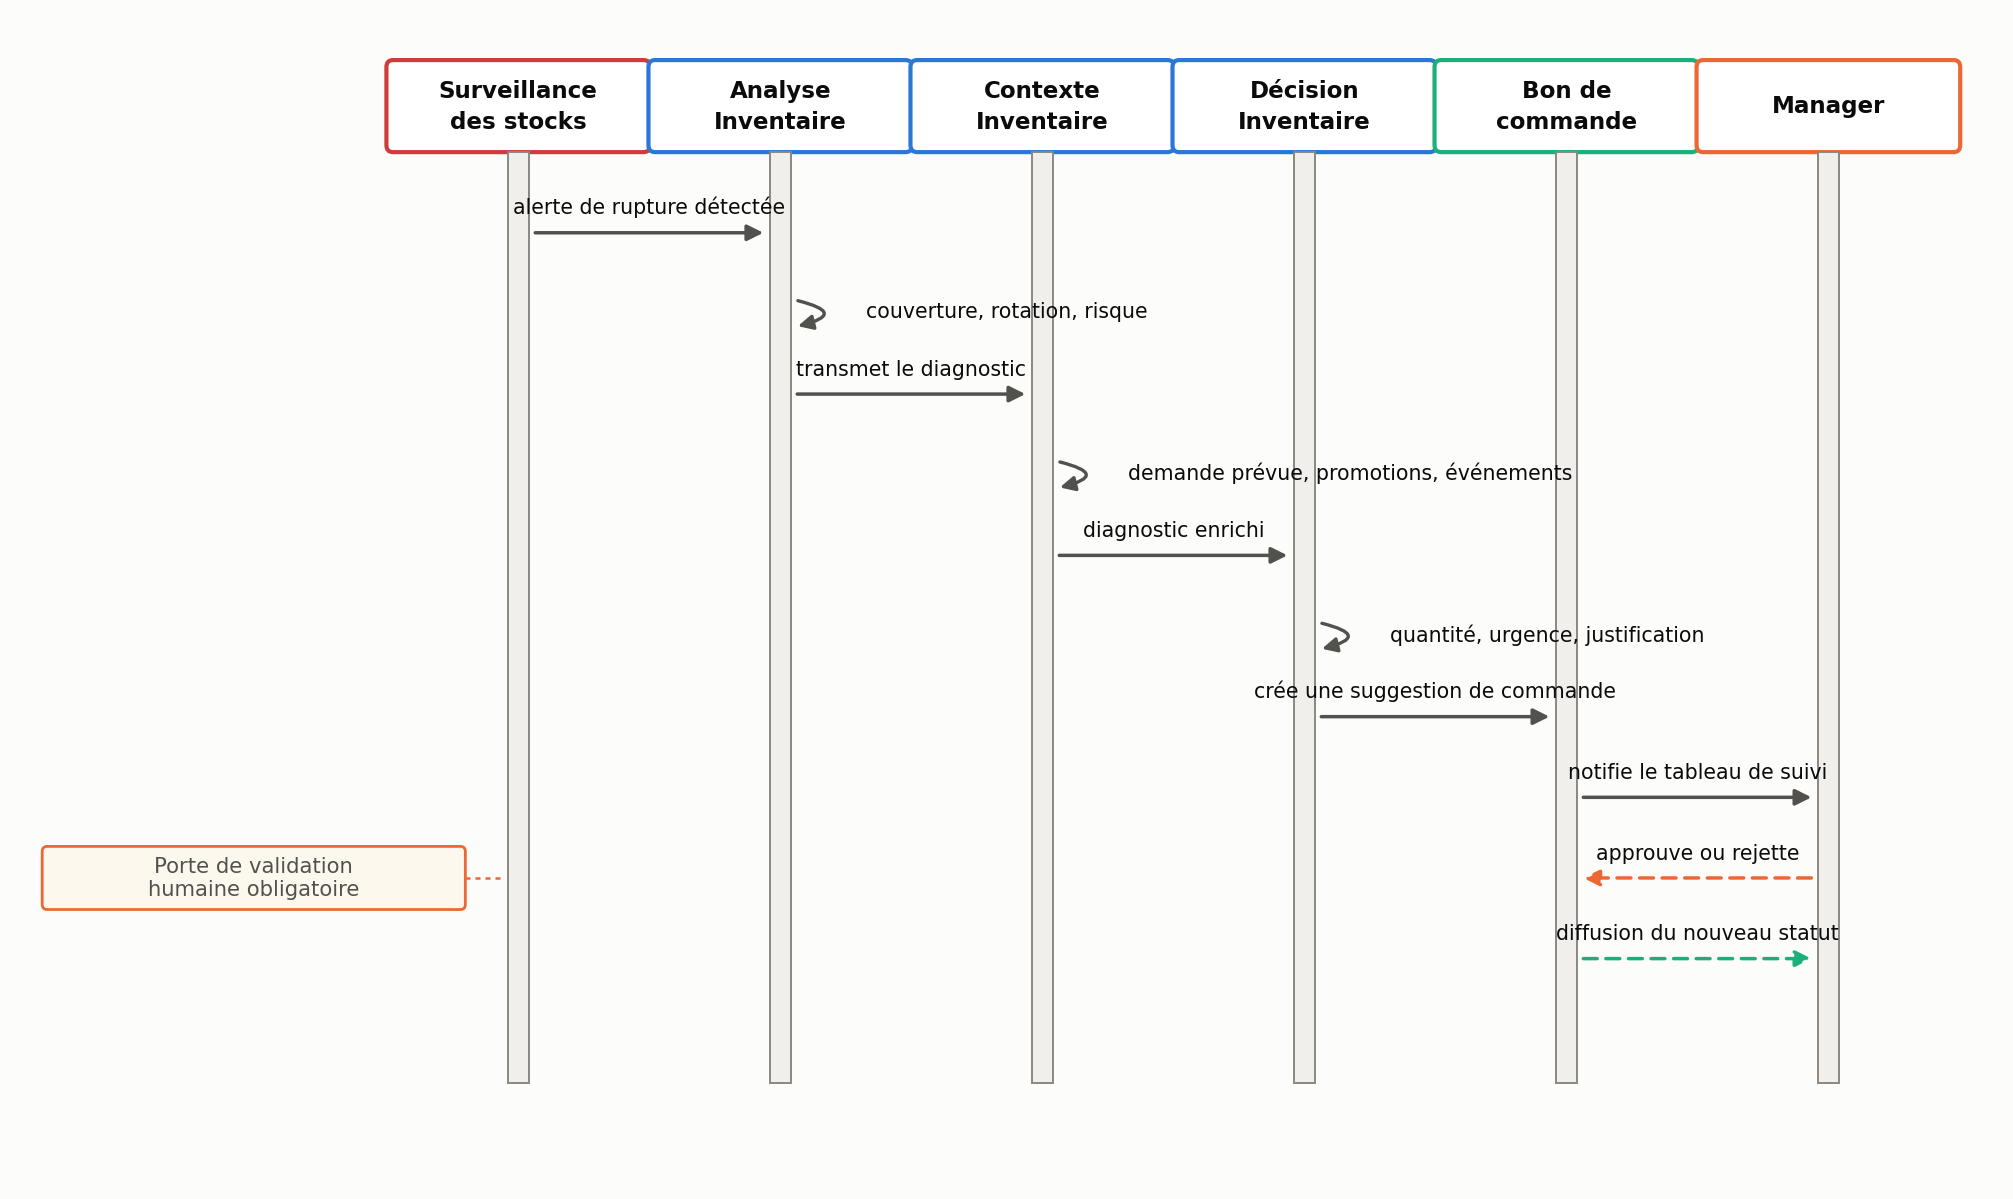
\includegraphics[width=\textwidth]{img/fig_sequence_reappro.png}
    \caption{Diagramme de séquence — de l'alerte de stock à la suggestion de commande}
    \label{fig:sequence-reappro-chap2}
\end{figure}

% ------------------------------------------------------------
\section{Production du plan de projet}
% ------------------------------------------------------------

La dernière tâche de la phase établit le plan de conduite du projet : découpage du travail, priorisation, planification et évaluation initiale des outils et techniques envisagés pour atteindre les objectifs analytiques \cite{chapman2000crisp}.

\subsection{Backlog priorisé des besoins}

Les exigences ont été décomposées en items de travail de deux natures :

\begin{itemize}[label=--]
    \item les \textbf{user stories} (US) \cite{cohn2004userstories}, qui expriment une valeur fonctionnelle directement perceptible par le conseiller ou le manager ;
    \item les \textbf{tâches techniques de fondation} (TF), qui construisent les briques nécessaires à leur réalisation : socle de données, agents, orchestration, évaluation.
\end{itemize}

La priorisation suit la méthode \textbf{MoSCoW} \cite{clegg1994moscow} et l'estimation de l'effort utilise des \textbf{points de complexité} suivant la suite de Fibonacci. Le backlog compte \textbf{82 user stories actives} et \textbf{46 tâches techniques}, pour un total planifié de \textbf{471 points} : 455 affectés aux itérations et 16 réservés aux activités transverses. La figure~\ref{fig:moscow-chap2} présente la répartition des user stories par niveau de priorité.

\begin{figure}[H]
    \centering
    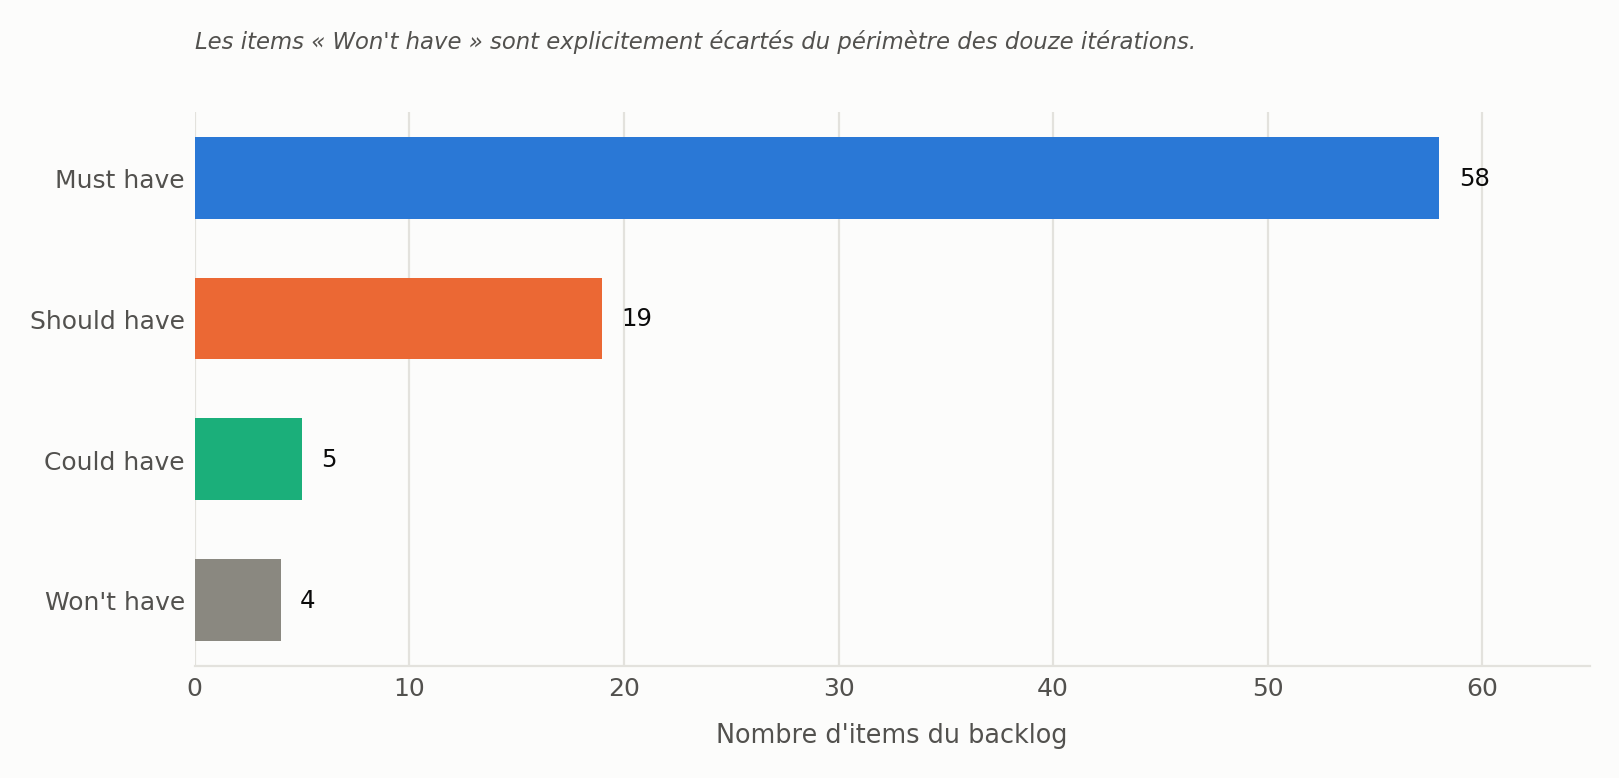
\includegraphics[width=0.86\textwidth]{img/fig_repartition_moscow.png}
    \caption{Répartition des user stories selon la priorisation MoSCoW}
    \label{fig:moscow-chap2}
\end{figure}

Le tableau~\ref{tab:backlog-us-chap2} présente le backlog priorisé, exprimé en récits utilisateur.

\begin{longtable}{|P{1.3cm}|P{7.8cm}|P{1.5cm}|P{1.2cm}|P{1.2cm}|}
\hline
\rowcolor{red!75}
\textcolor{white}{\textbf{ID}} &
\textcolor{white}{\textbf{User Story}} &
\textcolor{white}{\textbf{Priorité}} &
\textcolor{white}{\textbf{Points}} &
\textcolor{white}{\textbf{Itér.}} \\
\hline
\endhead
\hline
\endfoot
\hline
\endlastfoot
US-01 & En tant que conseiller, je veux me connecter à l'application afin d'accéder aux fonctionnalités correspondant à mon rôle et à ma boutique. & M & 3 & It. 2 \\
\hline
US-03 & En tant que conseiller, je veux consulter mon tableau de bord commercial afin de suivre ma performance actuelle. & M & 5 & It. 2 \\
\hline
US-06 & En tant que conseiller, je veux consulter la prévision de chiffre d'affaires de fin de journée afin d'anticiper l'atteinte de mon objectif. & M & 2 & It. 3 \\
\hline
US-11 & En tant que conseiller, je veux poser une question en langage naturel au Coach afin d'obtenir une assistance pendant la vente. & M & 5 & It. 3 \\
\hline
US-12 & En tant que conseiller, je veux recevoir la réponse du Coach progressivement afin de réduire le temps d'attente. & M & 3 & It. 3 \\
\hline
US-17 & En tant que conseiller, je veux consulter des scripts de vente contextualisés afin de mieux traiter les objections du client. & M & 3 & It. 4 \\
\hline
US-18 & En tant que conseiller, je veux des recommandations tenant compte de l'heure, du contexte et de l'état de la boutique afin d'obtenir un coaching pertinent. & M & 5 & It. 5 \\
\hline
US-20 & En tant que conseiller, je veux un produit de substitution lorsqu'un produit demandé est indisponible afin de ne pas perdre la vente. & M & 3 & It. 5 \\
\hline
US-37 & En tant que manager, je veux consulter les actions stratégiques prioritaires afin de décider des actions commerciales à lancer. & M & 3 & It. 6 \\
\hline
US-47 & En tant que manager, je veux voir chaque produit classé comme rupture, insuffisant, sain ou surstock afin d'identifier rapidement les risques. & M & 3 & It. 7 \\
\hline
US-58 & En tant que manager, je veux une décision d'approvisionnement par produit afin de savoir s'il faut commander, maintenir, surveiller ou accélérer. & M & 3 & It. 9 \\
\hline
US-76 & En tant que manager, je veux qu'une anomalie de vente déclenche automatiquement un cycle d'analyse afin d'obtenir une recommandation proactive. & M & 5 & It. 11 \\
\hline
US-83 & En tant que manager, je veux valider une recommandation escaladée afin d'autoriser sa diffusion. & M & 2 & It. 11 \\
\hline
US-64 & En tant que manager, je veux consulter les commandes suggérées dans un Kanban afin de suivre leur cycle de traitement. & M & 5 & It. 12 \\
\hline
\caption{Extrait du backlog priorisé des besoins}
\label{tab:backlog-us-chap2}
\end{longtable}

Quatre items ont été explicitement écartés du périmètre (\textit{Won't have}) : interface multilingue, application mobile native, intégration à un ERP réel et entraînement spécifique d'un modèle de langage propriétaire. Ces exclusions concentrent la capacité disponible sur les priorités \textit{Must} et \textit{Should}.

\subsection{Planification des itérations}

La distribution des items sur les douze itérations suit la logique de CRISP-DM : les premières itérations sont dominées par la compréhension et la préparation des données, les itérations intermédiaires par la modélisation, les dernières par l'évaluation et le déploiement. La figure~\ref{fig:planning-chap2} donne la vue calendaire de cette progression, et le tableau~\ref{tab:iterations-chap2} précise l'objectif de chaque itération.

\begin{figure}[H]
    \centering
    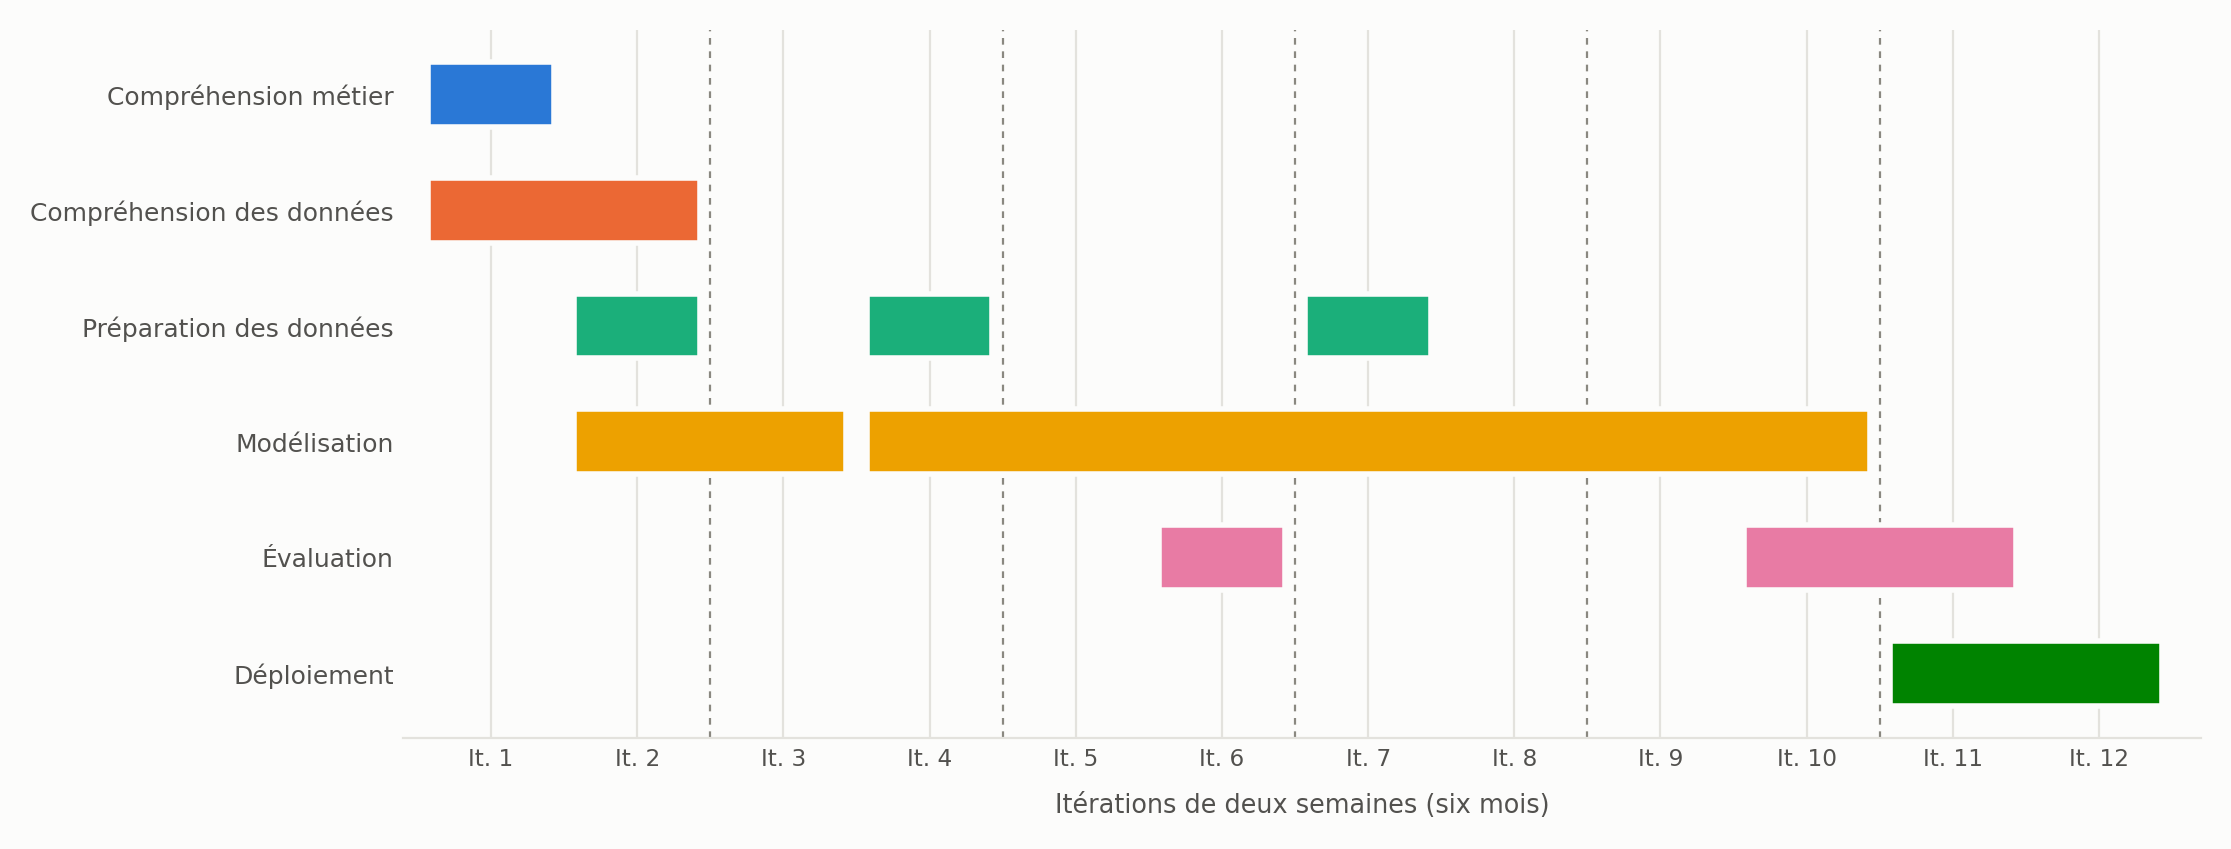
\includegraphics[width=\textwidth]{img/fig_planning_iterations.png}
    \caption{Planification des itérations par phase CRISP-DM dominante}
    \label{fig:planning-chap2}
\end{figure}

\begingroup
\setlength{\tabcolsep}{3pt}
\small

\begin{longtable}{|P{1.1cm}|P{1.8cm}|P{2.9cm}|P{6.4cm}|P{1.1cm}|}
\hline
\rowcolor{red!75}
\textcolor{white}{\textbf{Itér.}} &
\textcolor{white}{\textbf{Période}} &
\textcolor{white}{\textbf{Phase CRISP-DM}} &
\textcolor{white}{\textbf{Objectif de l'itération}} &
\textcolor{white}{\textbf{Pts}} \\
\hline
\endhead
\hline
\endfoot
\hline
\endlastfoot
It. 1 & M1, s. 1--2 & Compréhension métier et des données & Cadrer le périmètre, analyser les sources et poser le socle technique & 31 \\
\hline
It. 2 & M1, s. 3--4 & Préparation et modélisation & Versionner le schéma, enrichir les variables calendaires, premier moteur de prévision et tableau de bord & 33 \\
\hline
It. 3 & M2, s. 1--2 & Modélisation & Tableau de bord conseiller complet et assistant conversationnel en flux continu & 32 \\
\hline
It. 4 & M2, s. 3--4 & Préparation et modélisation & Base de connaissances métier et robustesse des appels aux modèles & 33 \\
\hline
It. 5 & M3, s. 1--2 & Modélisation & Coaching enrichi : scores, substitution, contexte, personnalisation & 34 \\
\hline
It. 6 & M3, s. 3--4 & Modélisation et évaluation & Supervision manager des ventes, agent de stratégie commerciale, interface responsive & 39 \\
\hline
It. 7 & M4, s. 1--2 & Préparation et modélisation & Domaine des stocks : état du portefeuille, couverture, rotation, paramètres de commande & 37 \\
\hline
It. 8 & M4, s. 3--4 & Modélisation & Prévision de la demande, contraintes fournisseurs, croisement des deux domaines & 30 \\
\hline
It. 9 & M5, s. 1--2 & Modélisation & Décision de réapprovisionnement et démarrage de l'orchestration & 36 \\
\hline
It. 10 & M5, s. 3--4 & Modélisation et évaluation & Orchestration avancée, observabilité, contrôle de conformité & 46 \\
\hline
It. 11 & M6, s. 1--2 & Évaluation et déploiement & Validation humaine, temps réel, boucle proactive, feedback & 50 \\
\hline
It. 12 & M6, s. 3--4 & Déploiement & Kanban des commandes, industrialisation, livrables de fin d'études & 54 \\
\hline
--- & It. 8--12 & Transverse & Tests, intégration continue, corrections & 16 \\
\hline
\caption{Planification des itérations et rattachement aux phases de CRISP-DM}
\label{tab:iterations-chap2}
\end{longtable}
\endgroup

La charge moyenne planifiée s'établit à 38 points par itération. Elle croît volontairement en fin de projet, comme le montre la figure~\ref{fig:charge-chap2} : les trois dernières itérations concentrent 150 points, soit près du tiers de la charge totale. Ce déséquilibre constitue le principal point de vigilance du plan et fonde le risque R7 du tableau~\ref{tab:risques-chap2} ; trois leviers d'ajustement sont prévus : la dépriorisation des items \textit{Should} des dernières itérations, la livraison du tableau de suivi des commandes en deux incréments, et la mobilisation de la réserve transverse pour absorber les débordements de test.

\begin{figure}[H]
    \centering
    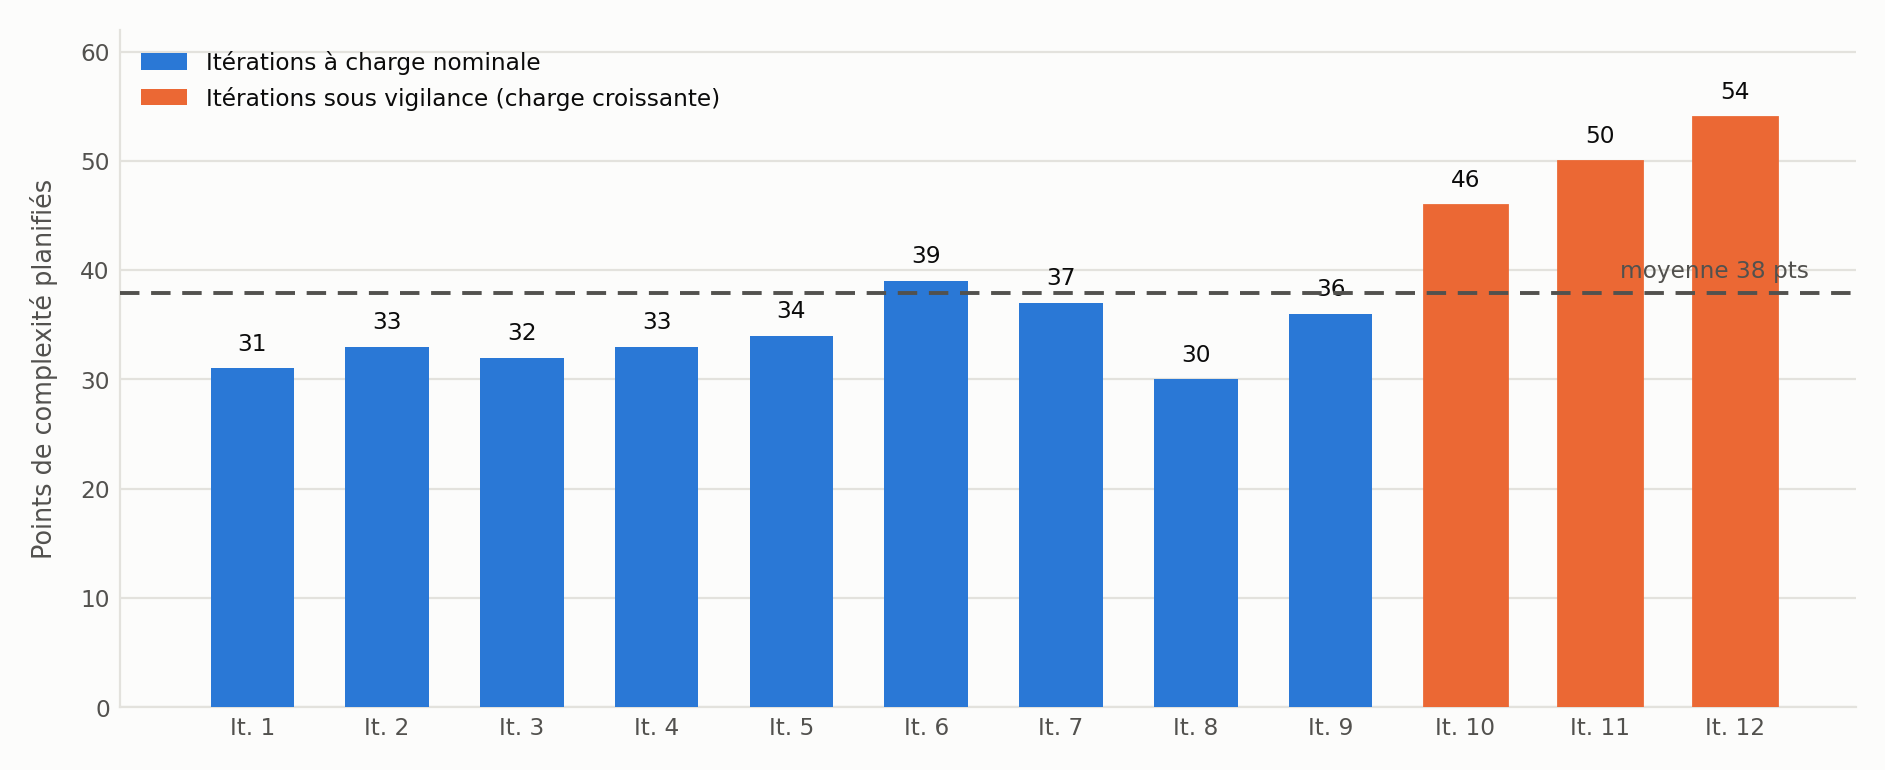
\includegraphics[width=\textwidth]{img/fig_charge_iterations.png}
    \caption{Charge planifiée par itération, en points de complexité}
    \label{fig:charge-chap2}
\end{figure}

\subsection{Évaluation initiale des outils et des techniques}

CRISP-DM demande, dès la phase de compréhension métier, une évaluation préliminaire des outils et techniques susceptibles d'atteindre les objectifs analytiques \cite{chapman2000crisp}. Cette évaluation n'engage pas le choix définitif — qui relève de la phase de modélisation, où il est confronté à la mesure — mais elle écarte d'emblée les options incompatibles avec les contraintes identifiées.

\begingroup
\setlength{\tabcolsep}{3pt}
\renewcommand{\arraystretch}{1.15}
\small

Le tableau~\ref{tab:outils-techniques-chap2} présente cette évaluation préliminaire, besoin par besoin.

\begin{longtable}{|P{2.6cm}|P{3.4cm}|P{4.0cm}|P{3.8cm}|}
\hline
\rowcolor{red!75}
\textcolor{white}{\textbf{Besoin technique}} &
\textcolor{white}{\textbf{Options envisagées}} &
\textcolor{white}{\textbf{Critère discriminant}} &
\textcolor{white}{\textbf{Orientation retenue}} \\
\hline
\endhead
\hline
\endfoot
\hline
\endlastfoot
Prévision de séries temporelles & Lissage exponentiel saisonnier \cite{holt2004forecasting,winters1960forecasting}, modèles à gradient boosté \cite{chen2016xgboost}, modèles de fondation pré-entraînés \cite{das2024timesfm} & Historique disponible, coût de calcul sur poste unique, erreur mesurée par rétro-test & Approche en cascade : modèle appris, repli statistique saisonnier, modèle de fondation optionnel \\
\hline
Orchestration multi-agents & Enchaînement programmé, cadre d'agents conversationnels \cite{wu2023autogen}, graphe d'états explicite & Contrôle du flux, exécution parallèle, reprise et traçabilité & Graphe d'états explicite, seul à rendre le flux vérifiable et journalisable \\
\hline
Modèles de langage & Fournisseur unique en ligne, modèles locaux, cascade multi-fournisseurs & Absence de budget, quotas, disponibilité, confidentialité & Cascade multi-fournisseurs avec repli local, sélection par rôle \\
\hline
Recherche de connaissances & Recherche lexicale \cite{robertson2009bm25}, recherche sémantique \cite{lewis2020rag}, recherche hybride \cite{gao2024rag} & Sensibilité aux références exactes et aux paraphrases & Recherche hybride avec reclassement métier et corpus de repli \\
\hline
Persistance & Base relationnelle, base documentaire, base vectorielle \cite{wang2021milvus} & Intégrité référentielle, agrégations analytiques, recherche sémantique & Base relationnelle pour le métier, base vectorielle pour le corpus \\
\hline
Temps réel & Interrogation périodique, événements serveur, WebSocket & Latence perçue, charge serveur, sens du flux & Événements serveur pour la réponse progressive, WebSocket pour les alertes et statuts \\
\hline
Évaluation de la qualité & Inspection manuelle, juge automatique \cite{zheng2023judge}, cadre d'évaluation de la génération augmentée \cite{es2024ragas}, mesure du retour humain & Reproductibilité, volume, coût & Combinaison : juge automatique hors chemin critique et mesure du taux d'acceptation \\
\hline
\caption{Évaluation initiale des outils et des techniques}
\label{tab:outils-techniques-chap2}
\end{longtable}
\endgroup

L'environnement de développement retenu à l'issue de cette évaluation est présenté au tableau~\ref{tab:env-logiciel-chap2}.

\begin{longtable}{|P{3.2cm}|P{3.8cm}|P{7.0cm}|}
\hline
\rowcolor{red!75}
\textcolor{white}{\textbf{Catégorie}} &
\textcolor{white}{\textbf{Technologie}} &
\textcolor{white}{\textbf{Rôle dans le projet}} \\
\hline
\endhead
\hline
\endfoot
\hline
\endlastfoot
Langage backend & Python 3.12 & Langage principal du backend et des agents \\
\hline
Framework backend & FastAPI / Uvicorn & API REST asynchrone, flux d'événements serveur et WebSockets \\
\hline
Orchestration agentique & LangGraph / LangChain & Graphe d'états multi-agents, exécution parallèle, état partagé \\
\hline
Base de données & PostgreSQL & Données métier organisées en schémas : ventes, stocks, approvisionnement, marché, transverse \\
\hline
Migrations & Alembic / SQLAlchemy & Versionnement du schéma, source de vérité unique de sa structure \\
\hline
Cache et temps réel & Redis & Cache applicatif, bus d'alertes, diffusion des événements de commande \\
\hline
Base vectorielle & Milvus & Recherche sémantique du corpus métier, avec repli local \\
\hline
Modèles de langage & Mistral, OpenRouter, Groq, Ollama & Cascade multi-fournisseurs avec sélection par rôle : analyse, décision, contrôle \\
\hline
Vectorisation & bge-m3 & Représentation multilingue des documents du corpus \\
\hline
Prévision & Modèle à gradient boosté, lissage exponentiel saisonnier, modèles de fondation optionnels & Prévision du chiffre d'affaires et de la demande, avec rétro-test et repli \\
\hline
Frontend & Angular (composants \textit{standalone}, \textit{Signals}), TypeScript & Interfaces conseiller et manager, responsive \\
\hline
Observabilité & Langfuse & Traçage des cycles d'agents : durées, erreurs, coûts \\
\hline
Tests & pytest & Tests unitaires et d'intégration \\
\hline
Conteneurisation & Docker / Docker Compose & Environnement reproductible \\
\hline
Gestion de versions & Git / GitHub, GitHub Actions & Versionnement et intégration continue \\
\hline
Environnement de développement & Visual Studio Code & Édition, exécution et débogage \\
\hline
Modélisation & draw.io / PlantUML & Diagrammes UML et d'architecture \\
\hline
\caption{Environnement logiciel retenu}
\label{tab:env-logiciel-chap2}
\end{longtable}

% ------------------------------------------------------------
\section*{Conclusion}
\addcontentsline{toc}{section}{Conclusion}
% ------------------------------------------------------------

Ce chapitre a conduit la première phase de CRISP-DM, la compréhension métier. Nous avons formulé sept objectifs métier et six critères auxquels l'entreprise jugera le résultat, puis dressé un état des lieux de la situation : ressources en données, en matériel et en compétences, acteurs humains et logiciels, exigences fonctionnelles regroupées en huit familles et exigences non fonctionnelles rattachées à la norme ISO/IEC 25010, hypothèses, contraintes, risques assortis de leurs parades, terminologie du domaine et analyse coûts-bénéfices.

Le point central du chapitre est la traduction de ces objectifs métier en huit objectifs de fouille de données, chacun associé à une métrique et à un critère de succès défini avant toute modélisation. Cette traduction, complétée par la matrice de traçabilité, garantit que chaque exigence exprimée se rattache à un objectif mesurable, et que l'évaluation conduite au chapitre~\ref{chap:evaluation} portera sur des seuils fixés à l'avance et non ajustés aux résultats obtenus.

Les besoins ont ensuite été formalisés en UML — diagramme de cas d'utilisation, fiches descriptives et diagrammes de séquence —, puis le plan de projet a été établi : backlog priorisé selon MoSCoW, planification des douze itérations rattachées aux phases de CRISP-DM, et évaluation initiale des outils et techniques compatibles avec les contraintes identifiées.

Le problème est désormais posé, borné et mesurable.

\textbf{Décision de fin de phase.} Les sept objectifs métier sont formulés, traduits en huit objectifs analytiques, et chacun est assorti d'une métrique et d'un critère de succès arrêté avant toute modélisation. Les ressources nécessaires sont identifiées et disponibles, les risques recensés et assortis de parades, et l'évaluation initiale des outils a écarté les options incompatibles avec les contraintes. Aucun objectif n'est dépourvu de réalisation prévue, aucune exigence n'est orpheline. La phase de compréhension des données est autorisée : elle fait l'objet du chapitre suivant, qui confrontera ces objectifs à la réalité des sources disponibles -- et pourra, conformément à la logique de retour propre à CRISP-DM, conduire à en réviser le périmètre.
